\RequirePackage[english=usenglishmax]{hyphsubst}
\documentclass[titlepage,letterpaper]{article}
\usepackage[utf8]{inputenc}
\usepackage[svgnames]{xcolor}
\usepackage{textcomp}
\usepackage{amsmath}
\usepackage[activate=true,final,tracking=true,kerning=true,spacing=true]{microtype}
\usepackage{natbib}
\usepackage{graphicx}
\usepackage{changepage}
\usepackage{indentfirst}
\usepackage{caption}
\usepackage{pgf}
\usepackage{tikz}
\usepackage{comment}
\usepackage{subcaption}
\usepackage{pgfplots}
\pgfplotsset{compat=newest}
\usepackage{mathtools}
\usepackage{kantlipsum}
\usepackage{natbib}
\usepackage{attachfile}
\usepackage{amsfonts}
\usepackage{amsmath}
\usepackage{placeins}
\usepackage{tcolorbox}
\usepackage{booktabs}
\setlength{\parindent}{4em}
\setlength{\parskip}{1em}
\usepackage{tabularx}
\usepackage[]{algorithm2e}
\setlength{\parindent}{3em}
\setlength{\parskip}{.75em}
%opening
\title{Sentiment Analysis in Text}
\author{Richard Lettich, Carmen Gaver, Bryce Taylor, Mary Grace Oster}
\date{Fall 2018}

\begin{document}

\maketitle

\begin{abstract}
This paper introduces an approach on how to predict sentiment from idioms and text using LSTM Neural Networks. In general, the neural networks tend to learn from loops and this allows the method to predict the correct sentiment with high success. Following an overview of LSTM Neural Networks, we show it's success rate on the Plutchik's Emotion data and the Twitter data. After showing what it will do on smaller data sets, we then show it used on raw scraped twitter data. \\
\end{abstract}

\section{Introduction}

The goal of this project is to create a method which will accurately analyze a given text and predict the correct emotion which is expressed in the text. For many companies there is a high need for programs which can analyze a customer review and determine the appropriate underlying sentiment. Customer satisfaction plays a huge role in how companies compete. Novak, Sparl, and Azman explain how ``increased service quality positively influences customer satisfaction", which in turn leads to better financial results through increased customer loyalty \cite{BusinessCustomerSatisfaction}. Therefore companies need to know how well they are doing, how satisfied are the customers, where the company can improve, and much more. The goal of this project is to create a method which can accurately assign emotion to a given sentence.

It should be stated that Chick-fil-A is a customer service oriented brand. They desire to potentially use the methods described in analysis as part of a larger project to discover how emotion relates to restaurant reviews in online comments and customer perception of service failure.

A spectrum of emotion (such as `satisfaction') would likely be best for this purpose. Since the goal is to determine what service failures and successes cause the strongest customer emotions and predict the former using the later, it would be best to rank the emotion quantitatively. Determining that long wait times make people unhappy would provide no novel information, but being able to say that people become an order of magnitude more upset over one service failure than another would beneficial as a tool of analysis. In addition, a spectrum of satisfaction would allow for better predictive capability when being used as a component of another analysis \cite{low}.

Secondly, it would be ideal to have a confidence value for the emotional prediction. If this sentiment analysis is used as part of another meta-tool, being able to provide estimate of confidence would allow the meta-tool to weigh the sentiment analysis appropriately with its other variables.

Succinctly, we can define what our desired result as follows: for a given snippet of text, give a numerical rating on a spectrum of a single (or possibly multiple) emotions; give a confidence score for this rating.

\section{Machine Learning}

Machine Learning is the process of using a data set of known variables to create an algorithm which will predict a response variable \cite{Statlearning}. There are many different machine learning methods, such as Quadratic Discriminant Analysis, Neural Networks, Ridge Regression, Logistic Regression, and much more \cite{Statlearning}. In this data set each sentence has an assigned emotion so the method will be a supervised learning method \cite{Statlearning}. Simply put a supervised learning method uses a data set which has both the predictor variable and the response variable to create an algorithm to predict the response variable \cite{Statlearning}. In this situation, the predictor variables are the sentences and the response variables are the emotions associated with each sentence \cite{Statlearning}. 

The machine learning process is fundamentally similar to regression. There is an algorithm which attempts to find optimal parameters \footnote{while the parameter of our model $f(x)$ is $x$, this is \emph{not} the parameter we are addressing} for the function f(x) to yield the best prediction. This algorithm is called the optimizer. For instance, if the optimizer was trying to produce a linear regression model, \[f(x) = mx + b \] The optimizer’s goal would be to find the most ideal values of parameters $m$ and $b$. 

While this task is not daunting for such a simple function, it becomes much more complex for larger models that may contain thousands of parameters. However, at the simplest level, the process involves three parts: the model $f(x)$ itself, an optimization algorithm $\alpha$,  and a loss function $\lambda$.

\subsection{Loss Function}

The loss function dignifies the error of the predictions made by the model. It takes two parameters: the evaluation of our model at any given point($y_p$), and the actual value of the function at that given point, as provided by the input data set ($y_p$). A simple error function would be magnitude of the distance from our prediction to what our actual value is
\[\lambda(y,y_p) =  |y - y_p| \]

The vast majority of loss functions are not so naive, generally averaging the loss of all $y_p$'s in some way, and weighing outliers to be greater, to prevent the 'perfection' of one point by lowering the general applicability of the model.

\subsection{Optimizer Function - Stochastic Gradient Descent}

In this project, we use the \textit{Adam} optimizer, which is a tuned up version of stochastic gradient descent optimization. As its name alludes to, stochastic gradient descent optimizes the model function by descending the gradient of the loss function. 

Before explaining what that means, it should be known that SGD optimizers assumes that if the loss function and model function are continuous \textit{enough}, then the mean value and rolle’s theorems \footnote{For a continuous function between two points the function must pass through the intermediate values; maxima and minima must occur at zero} still hold. 

From this, if we take any point on the loss function, we are able to extrapolate that if we were modify our parameters p (where $p = [m, b,...]$), going in the direction opposite of the gradient of the loss function with respect those parameters ($\frac{\partial\lambda}{\partial p}$), we would be able to continuously re-evaluate and lower our error until we reach a gradient near zero, indicating we hypothetically found model parameters which can not be improved.

SGD based optimizer functions find the gradient of this graph with respect to the optimization parameters (just $\frac{\partial\lambda}{\partial m}$ in this case). From this, they are able to accurately guess new parameters ($m$) in the direction of the opposite of the magnitude of the gradient which likely provide a lower error ($\lambda$). 

This process is iterative, and the change in parameter per iteration is called step size. Too large of a step size, and new parameter would `overshoot'. For instance if our $m$ was too small, `overshooting' would lead to it being too large.

	\begin{figure}[h]
	\centering 
	\label{fig:m_vs_error}
	\caption{M vs. Error}
	
\includegraphics[scale=.11]{error_function.eps}
	\vspace{-55pt}
	\end{figure}


\subsection{Caveats}
 
 Of course, the model isn't as simple as linear regression. With hundreds of thousands to millions of possible data points, some are bound to disagree on how to adjust parameters. In addition, not all critical points where minima occur are absolute minima, possibly leading to the optimizer  getting 'stuck' in a local minima. Moreover, saddle points occur in dimensions higher than two. The differences between SGD optimizers mainly concern to how work around these caveats while navigating the $\lambda$ graph.
 
\section{Sentiment Analysis}

In this project, ``sentiment analysis, also referred to as opinion mining, aims to automatically extract and classify sentiments, opinions, and emotions expressed in text" is performed on the Primary Emotion Data created by Lowri Williams \cite{lowriwilliams}. The purpose of Primary Emotion data set is to show the use-fullness of idioms in determining the emotion expressed in a given text. For example, ``we'd fight like cats and dogs", from this sentence we can deduce that whomever is speaking would have awful fights with someone else \cite{lowriwilliams}. The labeled sentences were determined by contributors looked at the sentences and rated their emotional content based on Plutchik's Wheel of Emotions and polarity categories \cite{lowriwilliams}. Sentiment classification problems often use polarity categories to represent and classify sentiment \cite{lowriwilliams}. Sentiment polarity can be positive, negative, and neutral. An example of sentiment polarity in the data is given by: "Mr.Jones was grinning from ear to ear"; that is a positive idiom; "I was bored to tears at work today" is a negative statement. After decided the polarity it is very simple to then pick an emotion for the sentence.\cite{lowriwilliams}. 

\section{Plutchik's Wheel of Emotion}

Plutchik's Wheel of Emotion, see Figure \ref{plutchikemotionwheell}, has eight basic emotions including: joy, trust, fear, surprise, sadness,disgust, anger, and anticipation. Each of the eight emotions has three levels of activation represented by color boldness. The emotion space is represented so that combinations of basic emotions derive secondary emotions. For example: joy+trust=love, anger+anticipation=aggression \cite{plutchik2001nature}.

The emotions on each leaf range in intensity. The emotions on the inner circle are the most intense and the emotions on the outer circle of each leaf are the least intense \cite{WheelofEmotion}. The emotions that fall between each leaf are a combination of each leaf's middle emotion \cite{WheelofEmotion}. For example, ``Trust + Fear = Submission". The Primary Emotion Data set has emotions from the middle of each leaf, the combinations emotions, and categories ``Neutral" and ``Ambiguous" \cite{lowriwilliams}.

\begin{figure}[ht]
	\center
	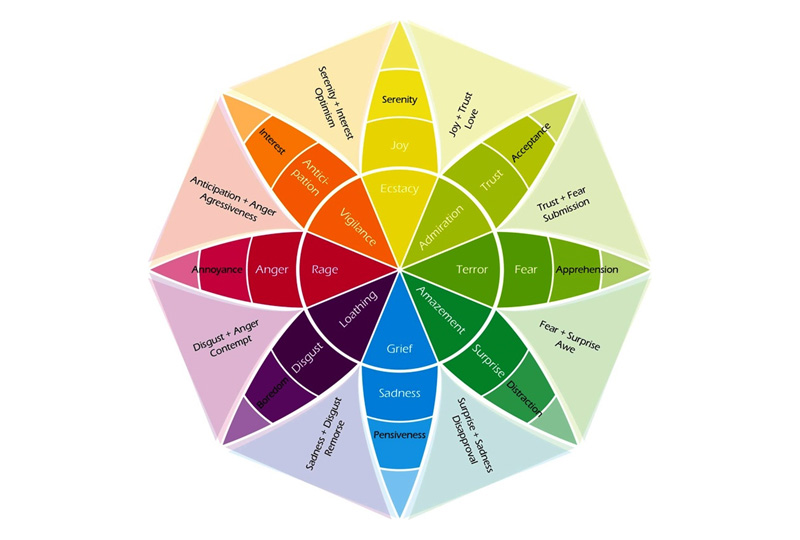
\includegraphics[width=4in]{PlutchikWheelOfEmotion.jpg}
	\caption{Plutchiks Wheel of Emotion \cite{WheelofEmotion}}
	\label{plutchikemotionwheel}
\end{figure}

\section{Primary Emotion Data}
Table \ref{PrimaryEmotionTable} gives a few examples of the sentences and labeled emotions in the Primary Emotion data. The Primary Emotion data set contains around $2425$ emotion labeled sentences. For this project the data will be used to develop a method which when given a text will assign the correct emotion to a given text. 
 
 \begin{center}
 	\begin{tabular}{ |c|c| } 
 		\hline
 		Emotion & Sentence \\
 		\hline \hline
 		Neutral & Don't let him pick a fight now, we're almost home. \\
 		\hline
 		Optimism &  You must sink your differences. \\
 		\hline
 		Aggression & We'd fight like cat and dog.  \\ 
 		\hline
 		Disgust & For God's sake bury the hatchet. \\
 		\hline
 	\end{tabular}
 	\captionof{table}{Primary Emotion Data}
 	\label{PrimaryEmotionTable}
 \end{center}

 
 Williams hypothesized that the use of idioms in sentiment analysis would increase the accuracy of predicting the correct emotion or category \cite{lowriwilliams}. Figure \ref{topsixgroups} shows a bar plot top six emotion groups, ranked by most frequently appearing groups in the data set. The emotion group ``Neutral" occurs the most, it makes up just over $20$ percent of the data set. 
 
% \begin{figure}[h!]
% 	\centering
% 	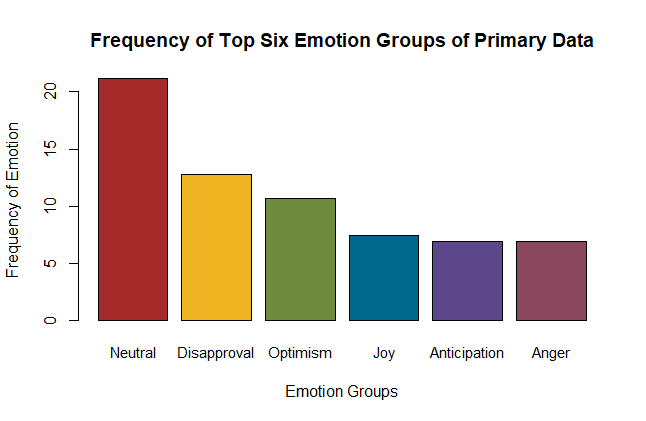
\includegraphics[width = 4.2in]{TopSixGroup1.png}
% 	\caption{Barplot of Frequency of Top Six Emotions in Primary Emotion Data}
% 	\label{TopSixGroup1}
% \end{figure}
 
% % Created by tikzDevice version 0.12 on 2018-11-30 19:07:14
% !TEX encoding = UTF-8 Unicode
\begin{document}
	content...
\begin{tikzpicture}[x=1pt,y=1pt]
\definecolor{fillColor}{RGB}{255,255,255}
\path[use as bounding box,fill=fillColor,fill opacity=0.00] (0,0) rectangle (361.35,361.35);
\begin{scope}
\path[clip] (  0.00,  0.00) rectangle (361.35,361.35);
\definecolor{drawColor}{RGB}{0,0,0}
\definecolor{fillColor}{RGB}{165,42,42}

\path[draw=drawColor,line width= 0.4pt,line join=round,line cap=round,fill=fillColor] ( 59.83, 63.68) rectangle ( 97.78,312.15);
\definecolor{fillColor}{RGB}{238,180,34}

\path[draw=drawColor,line width= 0.4pt,line join=round,line cap=round,fill=fillColor] (105.38, 63.68) rectangle (143.33,213.97);
\definecolor{fillColor}{RGB}{110,139,61}

\path[draw=drawColor,line width= 0.4pt,line join=round,line cap=round,fill=fillColor] (150.92, 63.68) rectangle (188.88,188.85);
\definecolor{fillColor}{RGB}{0,104,139}

\path[draw=drawColor,line width= 0.4pt,line join=round,line cap=round,fill=fillColor] (196.47, 63.68) rectangle (234.43,150.69);
\definecolor{fillColor}{RGB}{93,71,139}

\path[draw=drawColor,line width= 0.4pt,line join=round,line cap=round,fill=fillColor] (242.02, 63.68) rectangle (279.97,145.11);
\definecolor{fillColor}{RGB}{139,71,93}

\path[draw=drawColor,line width= 0.4pt,line join=round,line cap=round,fill=fillColor] (287.57, 63.68) rectangle (325.52,145.11);
\end{scope}
\begin{scope}
\path[clip] (  0.00,  0.00) rectangle (361.35,361.35);
\definecolor{drawColor}{RGB}{0,0,0}

\node[text=drawColor,anchor=base,inner sep=0pt, outer sep=0pt, scale=  1.00] at ( 78.81, 39.60) {Neutral};

\node[text=drawColor,anchor=base,inner sep=0pt, outer sep=0pt, scale=  1.00] at (169.90, 39.60) {Optimism};

\node[text=drawColor,anchor=base,inner sep=0pt, outer sep=0pt, scale=  1.00] at (215.45, 39.60) {Joy};

\node[text=drawColor,anchor=base,inner sep=0pt, outer sep=0pt, scale=  1.00] at (261.00, 39.60) {Anticipation};
\end{scope}
\begin{scope}
\path[clip] (  0.00,  0.00) rectangle (361.35,361.35);
\definecolor{drawColor}{RGB}{0,0,0}

\node[text=drawColor,anchor=base,inner sep=0pt, outer sep=0pt, scale=  1.20] at (192.68,332.61) {\bfseries Frequency of Top Six Emotion Groups of Primary Data};

\node[text=drawColor,anchor=base,inner sep=0pt, outer sep=0pt, scale=  1.00] at (192.68, 15.60) {Emotion Groups};

\node[text=drawColor,rotate= 90.00,anchor=base,inner sep=0pt, outer sep=0pt, scale=  1.00] at ( 10.80,186.67) {Frequency};
\end{scope}
\begin{scope}
\path[clip] (  0.00,  0.00) rectangle (361.35,361.35);
\definecolor{drawColor}{RGB}{0,0,0}

\path[draw=drawColor,line width= 0.4pt,line join=round,line cap=round] ( 49.20, 63.68) -- ( 49.20,298.56);

\path[draw=drawColor,line width= 0.4pt,line join=round,line cap=round] ( 49.20, 63.68) -- ( 43.20, 63.68);

\path[draw=drawColor,line width= 0.4pt,line join=round,line cap=round] ( 49.20,122.40) -- ( 43.20,122.40);

\path[draw=drawColor,line width= 0.4pt,line join=round,line cap=round] ( 49.20,181.12) -- ( 43.20,181.12);

\path[draw=drawColor,line width= 0.4pt,line join=round,line cap=round] ( 49.20,239.84) -- ( 43.20,239.84);

\path[draw=drawColor,line width= 0.4pt,line join=round,line cap=round] ( 49.20,298.56) -- ( 43.20,298.56);

\node[text=drawColor,rotate= 90.00,anchor=base,inner sep=0pt, outer sep=0pt, scale=  1.00] at ( 34.80, 63.68) {0};

\node[text=drawColor,rotate= 90.00,anchor=base,inner sep=0pt, outer sep=0pt, scale=  1.00] at ( 34.80,122.40) {5};

\node[text=drawColor,rotate= 90.00,anchor=base,inner sep=0pt, outer sep=0pt, scale=  1.00] at ( 34.80,181.12) {10};

\node[text=drawColor,rotate= 90.00,anchor=base,inner sep=0pt, outer sep=0pt, scale=  1.00] at ( 34.80,239.84) {15};

\node[text=drawColor,rotate= 90.00,anchor=base,inner sep=0pt, outer sep=0pt, scale=  1.00] at ( 34.80,298.56) {20};
\end{scope}
\end{tikzpicture}

\end{document}

 \begin{figure}[htb]
 		\centering
 		\resizebox{4in}{!}{% Created by tikzDevice version 0.12 on 2018-11-30 19:07:14
% !TEX encoding = UTF-8 Unicode
\begin{document}
	content...
\begin{tikzpicture}[x=1pt,y=1pt]
\definecolor{fillColor}{RGB}{255,255,255}
\path[use as bounding box,fill=fillColor,fill opacity=0.00] (0,0) rectangle (361.35,361.35);
\begin{scope}
\path[clip] (  0.00,  0.00) rectangle (361.35,361.35);
\definecolor{drawColor}{RGB}{0,0,0}
\definecolor{fillColor}{RGB}{165,42,42}

\path[draw=drawColor,line width= 0.4pt,line join=round,line cap=round,fill=fillColor] ( 59.83, 63.68) rectangle ( 97.78,312.15);
\definecolor{fillColor}{RGB}{238,180,34}

\path[draw=drawColor,line width= 0.4pt,line join=round,line cap=round,fill=fillColor] (105.38, 63.68) rectangle (143.33,213.97);
\definecolor{fillColor}{RGB}{110,139,61}

\path[draw=drawColor,line width= 0.4pt,line join=round,line cap=round,fill=fillColor] (150.92, 63.68) rectangle (188.88,188.85);
\definecolor{fillColor}{RGB}{0,104,139}

\path[draw=drawColor,line width= 0.4pt,line join=round,line cap=round,fill=fillColor] (196.47, 63.68) rectangle (234.43,150.69);
\definecolor{fillColor}{RGB}{93,71,139}

\path[draw=drawColor,line width= 0.4pt,line join=round,line cap=round,fill=fillColor] (242.02, 63.68) rectangle (279.97,145.11);
\definecolor{fillColor}{RGB}{139,71,93}

\path[draw=drawColor,line width= 0.4pt,line join=round,line cap=round,fill=fillColor] (287.57, 63.68) rectangle (325.52,145.11);
\end{scope}
\begin{scope}
\path[clip] (  0.00,  0.00) rectangle (361.35,361.35);
\definecolor{drawColor}{RGB}{0,0,0}

\node[text=drawColor,anchor=base,inner sep=0pt, outer sep=0pt, scale=  1.00] at ( 78.81, 39.60) {Neutral};

\node[text=drawColor,anchor=base,inner sep=0pt, outer sep=0pt, scale=  1.00] at (169.90, 39.60) {Optimism};

\node[text=drawColor,anchor=base,inner sep=0pt, outer sep=0pt, scale=  1.00] at (215.45, 39.60) {Joy};

\node[text=drawColor,anchor=base,inner sep=0pt, outer sep=0pt, scale=  1.00] at (261.00, 39.60) {Anticipation};
\end{scope}
\begin{scope}
\path[clip] (  0.00,  0.00) rectangle (361.35,361.35);
\definecolor{drawColor}{RGB}{0,0,0}

\node[text=drawColor,anchor=base,inner sep=0pt, outer sep=0pt, scale=  1.20] at (192.68,332.61) {\bfseries Frequency of Top Six Emotion Groups of Primary Data};

\node[text=drawColor,anchor=base,inner sep=0pt, outer sep=0pt, scale=  1.00] at (192.68, 15.60) {Emotion Groups};

\node[text=drawColor,rotate= 90.00,anchor=base,inner sep=0pt, outer sep=0pt, scale=  1.00] at ( 10.80,186.67) {Frequency};
\end{scope}
\begin{scope}
\path[clip] (  0.00,  0.00) rectangle (361.35,361.35);
\definecolor{drawColor}{RGB}{0,0,0}

\path[draw=drawColor,line width= 0.4pt,line join=round,line cap=round] ( 49.20, 63.68) -- ( 49.20,298.56);

\path[draw=drawColor,line width= 0.4pt,line join=round,line cap=round] ( 49.20, 63.68) -- ( 43.20, 63.68);

\path[draw=drawColor,line width= 0.4pt,line join=round,line cap=round] ( 49.20,122.40) -- ( 43.20,122.40);

\path[draw=drawColor,line width= 0.4pt,line join=round,line cap=round] ( 49.20,181.12) -- ( 43.20,181.12);

\path[draw=drawColor,line width= 0.4pt,line join=round,line cap=round] ( 49.20,239.84) -- ( 43.20,239.84);

\path[draw=drawColor,line width= 0.4pt,line join=round,line cap=round] ( 49.20,298.56) -- ( 43.20,298.56);

\node[text=drawColor,rotate= 90.00,anchor=base,inner sep=0pt, outer sep=0pt, scale=  1.00] at ( 34.80, 63.68) {0};

\node[text=drawColor,rotate= 90.00,anchor=base,inner sep=0pt, outer sep=0pt, scale=  1.00] at ( 34.80,122.40) {5};

\node[text=drawColor,rotate= 90.00,anchor=base,inner sep=0pt, outer sep=0pt, scale=  1.00] at ( 34.80,181.12) {10};

\node[text=drawColor,rotate= 90.00,anchor=base,inner sep=0pt, outer sep=0pt, scale=  1.00] at ( 34.80,239.84) {15};

\node[text=drawColor,rotate= 90.00,anchor=base,inner sep=0pt, outer sep=0pt, scale=  1.00] at ( 34.80,298.56) {20};
\end{scope}
\end{tikzpicture}

\end{document}
}
 		\caption{Top Six Emotion Groups}\label{topsixgroups}
 \end{figure}
 	
 %\clearpage
 
\section{Methods}

\subsection{Text Mining}
The goal of this project is to implement a method which when given a bit of text will sort the text into one of the emotions categories. The first step in this project, is to do some basic text mining. Text mining is the process of ``cleaning" a data set, most raw data will contain punctuation, capitalizations, quotes, tenses, and much more \cite{TextMining}. For most text analysis not all words are needed. Words like ``the", ``a", ``an", and others known as ``stopwords" are not important to build a model which will assign emotion or predict a star rating \cite{TextMining}. 

Once the data is clean, each sentence must be broken down into ``tokens". A token can be each sentence, each word, or even a set of words \cite{TextMining}. For this project each token represents a word in each sentence. 

\subsection{Term Frequency Matrix}
The next step in the project is to create a term frequency matrix. Specifically, a matrix with columns corresponding to the emotions we want to detect, and rows representing each word, the matrix itself will contain the number of times a word appears assigned to a given emotion. Since the data set contains over six thousand words the frequency matrix will be large.

\subsection{Adam Optimizer}
The Adam optimizer is the de facto successor to a RMSProp. In RMSProp initial values must be chosen for some variables in the optimization algorithm. This can lead to bias. The Adam optimizer improves upon RMSProp by correcting this bias in later calculations. In addition, while RMSProp calculates its effective step size using momentum, Adam implements a `Signal to Noise' method, changing it based on a smooth gradient moving average (moment estimation, $m_t$) and a moving variance estimation ($v_t$). This means the rate at which it navigates the gradient is a metaphorical function of confidence: the less steady the gradient, the slower it goes. The Adam optimizer has proved to produce consistently excellent results, therefore it was chosen as the benchmark optimizer for this project.

Below is a pseudo-code representation of the Adam optimizer (Algorithm $1$). Refer to Table \ref{adam_table} for explanation of the components and notation in the description of the optimizer.

\begin{table}[]
	\begin{adjustwidth}{-1in}{-1in}
		\centering
		\caption{Glossary of notation used in Adam optimizer}
		\label{adam_table}
		\begin{tabular}{lll}
			\hline
			& \textbf{Description}                                                   & \textbf{Elaboration}                                                                                                                                                                                                                                               \\ \hline
			\multicolumn{1}{|l}{$f(x)$}    & Objective function                                                     & \multicolumn{1}{l|}{\begin{tabular}[c]{@{}l@{}}The term to be minimized. This is not the model function.\\ If $g(x)$ function we wish to optimize, and $\lambda$ is\\ our loss function, $f(x) = \lambda \circ g(x)$. See eq. 1 \\ for clarification\end{tabular}} \\ \hline
			\multicolumn{1}{|l}{$\alpha$}  & Step Size                                                              & \multicolumn{1}{l|}{Size of increment of change of parameters per $t$.}                                                                                                                                                                                            \\ \hline
			\multicolumn{1}{|l}{$t$}       & Time                                                                   & \multicolumn{1}{l|}{\begin{tabular}[c]{@{}l@{}}Integer value to keep track of iteration of optimizer.\\ Pragmatically, the iterator variable of the optimizer for loop.\end{tabular}}                                                                              \\ \hline
			\multicolumn{1}{|l}{$\odot$}   & Component-Wise Multiplication                                          & \multicolumn{1}{l|}{\begin{tabular}[c]{@{}l@{}}$[a,b,c, ..] \odot [d, e,f,...] = [ad,be,cf,...]$, When a non\\ scalar $n$ value is raised to a power $p$, it implies\\  $n \odot n^{p-1}$\end{tabular}}                                                                      \\ \hline
			\multicolumn{1}{|l}{$m_t$}     & Moment  Estimation                                                     & \multicolumn{1}{l|}{\begin{tabular}[c]{@{}l@{}}Moving average of gradient -- a smoothed version of\\ the gradient function. Defined by first moment of \\ gradient.\end{tabular}}                                                                                  \\ \hline
			\multicolumn{1}{|l}{$v_t$}     & Variance Estimation                                                    & \multicolumn{1}{l|}{\begin{tabular}[c]{@{}l@{}}Variance of gradient function as defined by second\\  moment of gradient.\end{tabular}}                                                                                                                             \\ \hline
			\multicolumn{1}{|l}{$\theta$}  & \begin{tabular}[c]{@{}l@{}}Parameters of Model\\ Function\end{tabular} & \multicolumn{1}{l|}{Parameters of model. Earlier denoted $p$ and $m$.}                                                                                                                                                                                             \\ \hline
			\multicolumn{1}{|l}{$g_t$}     & Gradient                                                               & \multicolumn{1}{l|}{\begin{tabular}[c]{@{}l@{}}Gradient with respect to optimization parameters. \\ Earlier denoted  $\frac{\partial \lambda}{\partial p}$, more appropriately denoted $\nabla_\theta f(\theta)$\end{tabular}}                                   \\ \hline
			\multicolumn{1}{|l}{$\beta_1$} & Decay rate of $m_t$                                                    & \multicolumn{1}{l|}{\begin{tabular}[c]{@{}l@{}}Multiplied by previous $m_t$ each iteration($t$)  \\ before adding new information. \\ \\ Acceptable range [0,1), Default .9\end{tabular}}                                                                           \\ \hline
			\multicolumn{1}{|l}{$\beta_2$} & Decay rate of $v_t$                                                    & \multicolumn{1}{l|}{\begin{tabular}[c]{@{}l@{}}Multiplied by previous $v_t$ each iteration($t$) \\ before taking into account  \\ \\ Acceptable range: [0,1), Default .999\end{tabular}}                                                                           \\ \hline
		\end{tabular}
	\end{adjustwidth}
\end{table}

\newcommand{\assn}{\mathrel{{:}{=}}}

\begin{algorithm}[]
	\label{adam_alg}
	\KwData{$\theta_0$, $f(x)$ (initial function parameters, unoptimized objective function), }
	\textbf{Initialize variables}:
	$\{m_0,V_0,t\} = 0$\;
	\vspace{3.5mm}
	\While{\text{model is not fitted}}{
		\begin{align*}
		t &\assn t +  1\\ 
		g_t &\assn \nabla_\theta f\left(\theta_{t-1}\right)\;  \hspace{2mm} \text{Find actual gradient. }\\
		m_t &\assn \beta_1 m_{t-1} + (1-\beta_1)g_t\\
		&\text{Assign new gradient moving average, where previous} \\
		&\text{gradients have weight} \frac{\beta_1}{1} \\
		v_t &\assn \beta_2 m_{t-1} + (1-\beta_1)g_t^2 \\
		&\text{Assign a new moving variance estimation in the same manner,}\\
		&\text{but instead using } \beta_2\\
		\widehat{m_t} &\assn \frac{m_t}{1-\beta_1^t}\\
		\widehat{v_t} &\assn \frac{v_t}{1-\beta_2^t}\\
		&\text{Bias results from where we initiated } v_t \text{ with zero. The last two}\\
		&\text{statements correct that bias. See Adam paper.}\\
		\theta_t &\assn \theta_{t-1} - \alpha\frac{ \widehat{m_t}}{\sqrt{v_t} + \epsilon}\\
		& \text{Update the parameters going in the opposite direction of our new}\\
		& \text{calculated gradient average. Weigh update by dividing by } \sqrt{\widehat{v_t}}, \\
		& \text{(more noise, lower effective step size.)}
		\end{align*}
	}
	\vspace{3.5mm}
	\caption{Pseudo-code representation of Adam optimizer. The $\mathrel{{:}{=}}$ ligature  represents assignment.}
\end{algorithm}

\paragraph{Gradient} - The gradient of a function $\nabla_\theta f(\theta)$ evaluated at point $\theta$ is by definition the direction of steepest ascent at point $\theta$. We use this, as we are trying to reduce our inaccuracy/loss by moving in the direction of steepest \textit{descent} \mbox{(i.e. $-\nabla_\theta f(\theta)$)}. 

\paragraph{Gradient Moving Average}

The Adam optimizer does not just naively use the gradient itself, but instead smooths it using the exponential moving average as originally described by J. Stuart Hunter\cite{EMA}. This formula gives a much less noisy curve to descend, and helps prevent the optimizer from plateauing in local minima. Although used recursively here, a non recursive equivalent is given by
\[m_t = \sum_{t=0}^{t_f} \left(1-\beta_1\right) \beta_1^{t_f-t}\nabla_\theta f\left(\theta_{t}\right)^2\]
Although purely semantic, in the original EMA formula, \(\beta_1\) and \(\left(1-\beta_1\right)\) are switched.


\paragraph{Moving Variance}
The moving variance is used to modulate the learning rate of the function, depending on how noisy the slope is. For an intuitive sense, recall that standard deviation is:
\[\sigma = \sqrt{\sum \left(x_n - \bar{x}\right)}\]
If we replace \(x_n\) with \ \(\nabla_\theta f(\theta)\), and \(\bar{x}\) with a gradient of \(\vec{0}\), we get \footnote{\(f\left(\theta_{t}\right)^2 \implies \) component wise multiplication}
\[\sigma = \sqrt{\sum \left(\nabla_\theta f(\theta)\right)^2}\]
Applying the same exponential moving average to this `variance from the zero gradient' yields a moving average in the same manner of the moving average of the gradient. Albeit, the variance is more conservative, as \(\beta_2\) is typically larger than \(\beta_1\).

\subsection{Model Layers}

A different approach was used for each model. Historically, Bidirectional LSTM has shown better results for textual analysis. However, in testing, it performed equivalently or worst than regular LSTM, and significantly increased time to convergence.

However, implementing Bi-directional LSTM on the idiom data has yielded a significant boost, raising accuracy approximately 5\% over regular LSTM.

\subsection{Dropout Technique}
Dropout is a regularization technique for the Long Short Term Memory Neural Networks. It is a new approach that randomly picks neurons to be dropped from the training network \cite{nielsen2015neural}. Those neurons are completely neglected. The goal of using this approach is to keep the neural network from overfitting to the training set. The dropout rate that is used and experimented with is between 20-50\% \cite{nielsen2015neural}.

\section{Positive and Negative Groups}

For this project, we first ran our method on Primary Emotion Data \cite{lowriwilliams}, then we ran it on Twitter data to see if the method would work on both sets and accurately predict the underlying emotion of a text. In both cases the data was broken into two groups, positive and negative. Once the data was labeled as positive and negative, the data was then split into a training set and a testing or validation set. Next the data goes through the LSTM method, which is programmed to go through each element of the data set and learn the appropriate response variable. In this project the LSTM network loops through each sentence and the corresponding emotion category and then continues through each sentence. This LSTM network learns the proportion of each emotion category. Once the LSTM network has gone through the entire training data set, it will go through the test data set. The network will predict the same proportion of emotion categories as represented in the training data set. 

\section{Results}

\subsection{Primary Emotion Data Results}
The Primary Emotion Data positive group contained the categories joy, love, optimism, trust, and awe; in the negative group we have anger, disgust, sadness, aggression, contempt, disapproval, and remorse. The rest of the emotion groups are left out since they do not fall into either positive or negative categorizations.

The results from training set, which was made up of $80$ percent of the data, had an accuracy of around $89$ percent. The testing set was made up of the remaining $20$ percent of the data and had an accuracy of $74$ percent. The gap in the training and testing accuracy is not a good sign, as the gap suggests that the method is over-fitting to  the training set. Put more simply, the method is learning the patterns of the training data set, rather than learning the overall spread or picture of the data. Consequently the method can accurately predict the training set, but it makes less accurate predictions for data it has not yet seen.

Figure \ref{primemresult} is a barplot of the results for the Primary Emotion Data testing set. There is a bar for positive predictions and a bar for negative predictions. The light blue shows the percent of correct predictions for both categories. The dark blue bar shows the percent of False Negatives, or sentences which should have been classified as positive for the positive bar, or negative in the negative bar. This barplot tells us how accurate the model is, which group the model is predicting accurately, and which group the model isn't predicting accurately. For the Primary Emotion data the model is most accurately predicting the positive emotions, meanwhile it isn't doing as well with the negative emotion group. We want the model to do a better job of predicting negative sentiment. 

Companies want to know which areas they need to improve. A big part of that process is finding out where the company is going wrong with the customer. This information is found in reviews from the customer, whether through some social media website, Yelp!, or reviews posted directly to the company. At some point the company is going to see the comment, tweet, or review and have to analyze it. However a problem with this is the volume of reviews a company, especially a big chain restaurant will recieve. A model like the one developed in this project could go through a large set of reviews and tell the company which reviews should be looked at, or which reviews are the most important. In other words, the model used in this project could tell a company which reviews are the most negative and should be investigated further.   

%\begin{figure}[h!]
%	\center
%	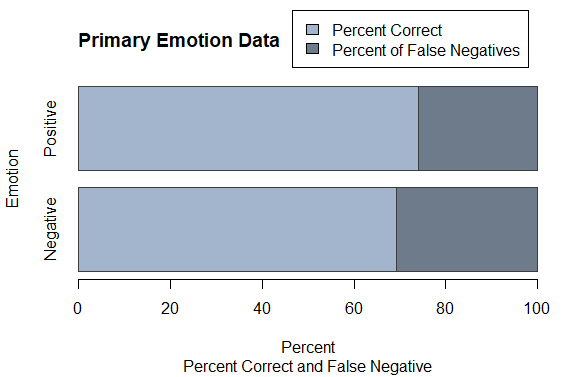
\includegraphics[width = 3.5in]{BarPlotPrimaryResults.png}
%	\caption{Barplot of Results of Primary Emotion Data, Positive and Negative Categories}
%	\label{bpprimem}
%\end{figure}

 \begin{figure}[htb]
	\centering
	\resizebox{4in}{!}{% Created by tikzDevice version 0.12 on 2018-12-01 10:49:27
% !TEX encoding = UTF-8 Unicode

\begin{tikzpicture}[x=1pt,y=1pt]
\definecolor{fillColor}{RGB}{255,255,255}
\path[use as bounding box,fill=fillColor,fill opacity=0.00] (0,0) rectangle (361.35,361.35);
\begin{scope}
\path[clip] (  0.00,  0.00) rectangle (361.35,361.35);
\definecolor{drawColor}{gray}{0.24}
\definecolor{fillColor}{RGB}{162,181,205}

\path[draw=drawColor,line width= 0.4pt,line join=round,line cap=round,fill=fillColor] ( 49.20, 70.49) rectangle (248.09,176.11);
\definecolor{fillColor}{RGB}{110,123,139}

\path[draw=drawColor,line width= 0.4pt,line join=round,line cap=round,fill=fillColor] (248.09, 70.49) rectangle (336.12,176.11);
\definecolor{fillColor}{RGB}{162,181,205}

\path[draw=drawColor,line width= 0.4pt,line join=round,line cap=round,fill=fillColor] ( 49.20,197.24) rectangle (261.74,302.86);
\definecolor{fillColor}{RGB}{110,123,139}

\path[draw=drawColor,line width= 0.4pt,line join=round,line cap=round,fill=fillColor] (261.74,197.24) rectangle (336.12,302.86);
\end{scope}
\begin{scope}
\path[clip] (  0.00,  0.00) rectangle (361.35,361.35);
\definecolor{drawColor}{RGB}{0,0,0}

\node[text=drawColor,rotate= 90.00,anchor=base,inner sep=0pt, outer sep=0pt, scale=  1.00] at ( 34.80,123.30) {Negative};

\node[text=drawColor,rotate= 90.00,anchor=base,inner sep=0pt, outer sep=0pt, scale=  1.00] at ( 34.80,250.05) {Positive};
\end{scope}
\begin{scope}
\path[clip] (  0.00,  0.00) rectangle (361.35,361.35);
\definecolor{drawColor}{RGB}{0,0,0}

\path[draw=drawColor,line width= 0.4pt,line join=round,line cap=round] (184.39,345.10) rectangle (328.92,309.10);
\definecolor{fillColor}{RGB}{162,181,205}

\path[draw=drawColor,line width= 0.4pt,line join=round,line cap=round,fill=fillColor] (193.39,336.10) rectangle (200.59,330.10);
\definecolor{fillColor}{RGB}{110,123,139}

\path[draw=drawColor,line width= 0.4pt,line join=round,line cap=round,fill=fillColor] (193.39,324.10) rectangle (200.59,318.10);

\node[text=drawColor,anchor=base west,inner sep=0pt, outer sep=0pt, scale=  1.00] at (209.59,329.66) {Percent Correct};

\node[text=drawColor,anchor=base west,inner sep=0pt, outer sep=0pt, scale=  1.00] at (209.59,317.66) {Percent of False Negatives};

\node[text=drawColor,anchor=base west,inner sep=0pt, outer sep=0pt, scale=  1.20] at ( 49.20,332.61) {\bfseries Results of Primary Emotion Data};

\node[text=drawColor,anchor=base,inner sep=0pt, outer sep=0pt, scale=  1.00] at (192.68,  3.60) {Percent Correct and False Negative};

\node[text=drawColor,anchor=base,inner sep=0pt, outer sep=0pt, scale=  1.00] at (192.68, 15.60) {Percent};

\node[text=drawColor,rotate= 90.00,anchor=base,inner sep=0pt, outer sep=0pt, scale=  1.00] at ( 10.80,186.67) {Emotion};
\end{scope}
\begin{scope}
\path[clip] (  0.00,  0.00) rectangle (361.35,361.35);
\definecolor{drawColor}{RGB}{0,0,0}

\path[draw=drawColor,line width= 0.4pt,line join=round,line cap=round] ( 49.20, 61.20) -- (336.15, 61.20);

\path[draw=drawColor,line width= 0.4pt,line join=round,line cap=round] ( 49.20, 61.20) -- ( 49.20, 55.20);

\path[draw=drawColor,line width= 0.4pt,line join=round,line cap=round] (106.59, 61.20) -- (106.59, 55.20);

\path[draw=drawColor,line width= 0.4pt,line join=round,line cap=round] (163.98, 61.20) -- (163.98, 55.20);

\path[draw=drawColor,line width= 0.4pt,line join=round,line cap=round] (221.37, 61.20) -- (221.37, 55.20);

\path[draw=drawColor,line width= 0.4pt,line join=round,line cap=round] (278.76, 61.20) -- (278.76, 55.20);

\path[draw=drawColor,line width= 0.4pt,line join=round,line cap=round] (336.15, 61.20) -- (336.15, 55.20);

\node[text=drawColor,anchor=base,inner sep=0pt, outer sep=0pt, scale=  1.00] at ( 49.20, 39.60) {0};

\node[text=drawColor,anchor=base,inner sep=0pt, outer sep=0pt, scale=  1.00] at (106.59, 39.60) {20};

\node[text=drawColor,anchor=base,inner sep=0pt, outer sep=0pt, scale=  1.00] at (163.98, 39.60) {40};

\node[text=drawColor,anchor=base,inner sep=0pt, outer sep=0pt, scale=  1.00] at (221.37, 39.60) {60};

\node[text=drawColor,anchor=base,inner sep=0pt, outer sep=0pt, scale=  1.00] at (278.76, 39.60) {80};

\node[text=drawColor,anchor=base,inner sep=0pt, outer sep=0pt, scale=  1.00] at (336.15, 39.60) {100};
\end{scope}
\end{tikzpicture}
}
	\caption{Barplot of Primary Emotion Results}\label{primemresult}
\end{figure}

\subsection{Labeled Twitter Data Results}

The Twitter data consists of about $40,000$ tweets, assigned emotion, and user identification. There are some cases of multiple tweets from the same person. The emotion categories are empty, sadness, enthusiasm, neutral, worry, love, fun, hate, happiness, surprise, and boredom. The twitter data was split into positive and negative categories. The positive category contains the emotion groups enthusiasm, love, and happiness. The negative category contains the emotion groups sadness and hate. The other emotions are left out since they do not fall into completely positive or negative categories. 

The training set contained $90$ percent of the data and had an accuracy of $82.29$ percent. The testing set contained the remaining $10$ percent of the data and had an accuracy of $83.3$ percent. The testing accuracy was actually higher than the training accuracy which tells us the method was not over-fitting to the training data. The testing set contained a higher percentage of the data compared to the Primary Emotion data since the Twitter data is a bigger data set, and $10$ of the data was more than and adequate size for testing the method. 

Figure \ref{lbtwitresult} is a barplot containing the results of the testing set for the Twitter data. There is a bar for both the negative and positive results. The light green shows the percent of correct predictions for each group. The dark green bar shows the percent of false negatives for each group. In other words, the percent of sentences that should have been predicted to be positive in the positive bar, or negative in the negative bar. From this barplot we can see that the model is doing a great job of predicting negative sentiment in the Twitter data but not as well of a job with the positive sentiment. However the percent of correctly predicted positive sentiment for the Twitter data is about the same as the percent of correctly predicted positive sentiment in the Primary Emotion data. We want the model to accurately find the negative sentiment in tweets, since that is what companies are interested in. Most companies want to know which areas they are succeeding in, but they need to know which areas they can improve. If our model can accurately find negative sentiment in a tweet or a comment, we can then make recommendations based on that output about which reviews the company should be taking seriously. 

%\begin{figure}[h!]
%	\centering
%	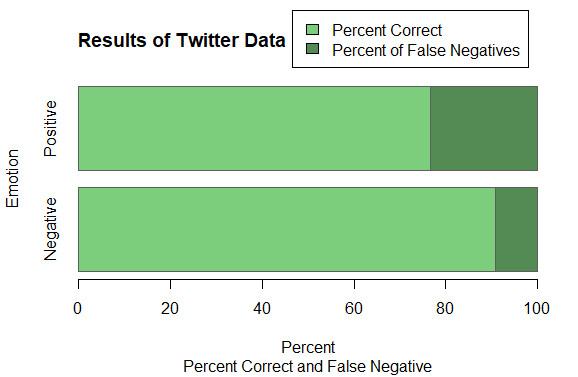
\includegraphics[width = 3.5in]{BarPlotTwitterResults.png}
%	\caption{Barplot of Results of Twitter Data, Positive and Negative Categories}
%\end{figure}

\begin{figure}[htb]
	\centering
	\resizebox{4in}{!}{% Created by tikzDevice version 0.12 on 2018-12-01 10:48:48
% !TEX encoding = UTF-8 Unicode
\begin{tikzpicture}[x=1pt,y=1pt]
\definecolor{fillColor}{RGB}{255,255,255}
\path[use as bounding box,fill=fillColor,fill opacity=0.00] (0,0) rectangle (361.35,361.35);
\begin{scope}
\path[clip] (  0.00,  0.00) rectangle (361.35,361.35);
\definecolor{drawColor}{gray}{0.37}
\definecolor{fillColor}{RGB}{124,205,124}

\path[draw=drawColor,line width= 0.4pt,line join=round,line cap=round,fill=fillColor] ( 49.20, 70.49) rectangle (309.64,176.11);
\definecolor{fillColor}{RGB}{84,139,84}

\path[draw=drawColor,line width= 0.4pt,line join=round,line cap=round,fill=fillColor] (309.64, 70.49) rectangle (336.12,176.11);
\definecolor{fillColor}{RGB}{124,205,124}

\path[draw=drawColor,line width= 0.4pt,line join=round,line cap=round,fill=fillColor] ( 49.20,197.24) rectangle (269.00,302.86);
\definecolor{fillColor}{RGB}{84,139,84}

\path[draw=drawColor,line width= 0.4pt,line join=round,line cap=round,fill=fillColor] (269.00,197.24) rectangle (336.12,302.86);
\end{scope}
\begin{scope}
\path[clip] (  0.00,  0.00) rectangle (361.35,361.35);
\definecolor{drawColor}{RGB}{0,0,0}

\node[text=drawColor,rotate= 90.00,anchor=base,inner sep=0pt, outer sep=0pt, scale=  1.00] at ( 34.80,123.30) {Negative};

\node[text=drawColor,rotate= 90.00,anchor=base,inner sep=0pt, outer sep=0pt, scale=  1.00] at ( 34.80,250.05) {Positive};
\end{scope}
\begin{scope}
\path[clip] (  0.00,  0.00) rectangle (361.35,361.35);
\definecolor{drawColor}{RGB}{0,0,0}

\path[draw=drawColor,line width= 0.4pt,line join=round,line cap=round] (184.39,345.10) rectangle (328.92,309.10);
\definecolor{fillColor}{RGB}{124,205,124}

\path[draw=drawColor,line width= 0.4pt,line join=round,line cap=round,fill=fillColor] (193.39,336.10) rectangle (200.59,330.10);
\definecolor{fillColor}{RGB}{84,139,84}

\path[draw=drawColor,line width= 0.4pt,line join=round,line cap=round,fill=fillColor] (193.39,324.10) rectangle (200.59,318.10);

\node[text=drawColor,anchor=base west,inner sep=0pt, outer sep=0pt, scale=  1.00] at (209.59,329.66) {Percent Correct};

\node[text=drawColor,anchor=base west,inner sep=0pt, outer sep=0pt, scale=  1.00] at (209.59,317.66) {Percent of False Negatives};

\node[text=drawColor,anchor=base west,inner sep=0pt, outer sep=0pt, scale=  1.20] at ( 49.20,332.61) {\bfseries Results of Twitter Data};

\node[text=drawColor,anchor=base,inner sep=0pt, outer sep=0pt, scale=  1.00] at (192.68,  3.60) {Percent Correct and False Negative};

\node[text=drawColor,anchor=base,inner sep=0pt, outer sep=0pt, scale=  1.00] at (192.68, 15.60) {Percent};

\node[text=drawColor,rotate= 90.00,anchor=base,inner sep=0pt, outer sep=0pt, scale=  1.00] at ( 10.80,186.67) {Emotion};
\end{scope}
\begin{scope}
\path[clip] (  0.00,  0.00) rectangle (361.35,361.35);
\definecolor{drawColor}{RGB}{0,0,0}

\path[draw=drawColor,line width= 0.4pt,line join=round,line cap=round] ( 49.20, 61.20) -- (336.15, 61.20);

\path[draw=drawColor,line width= 0.4pt,line join=round,line cap=round] ( 49.20, 61.20) -- ( 49.20, 55.20);

\path[draw=drawColor,line width= 0.4pt,line join=round,line cap=round] (106.59, 61.20) -- (106.59, 55.20);

\path[draw=drawColor,line width= 0.4pt,line join=round,line cap=round] (163.98, 61.20) -- (163.98, 55.20);

\path[draw=drawColor,line width= 0.4pt,line join=round,line cap=round] (221.37, 61.20) -- (221.37, 55.20);

\path[draw=drawColor,line width= 0.4pt,line join=round,line cap=round] (278.76, 61.20) -- (278.76, 55.20);

\path[draw=drawColor,line width= 0.4pt,line join=round,line cap=round] (336.15, 61.20) -- (336.15, 55.20);

\node[text=drawColor,anchor=base,inner sep=0pt, outer sep=0pt, scale=  1.00] at ( 49.20, 39.60) {0};

\node[text=drawColor,anchor=base,inner sep=0pt, outer sep=0pt, scale=  1.00] at (106.59, 39.60) {20};

\node[text=drawColor,anchor=base,inner sep=0pt, outer sep=0pt, scale=  1.00] at (163.98, 39.60) {40};

\node[text=drawColor,anchor=base,inner sep=0pt, outer sep=0pt, scale=  1.00] at (221.37, 39.60) {60};

\node[text=drawColor,anchor=base,inner sep=0pt, outer sep=0pt, scale=  1.00] at (278.76, 39.60) {80};

\node[text=drawColor,anchor=base,inner sep=0pt, outer sep=0pt, scale=  1.00] at (336.15, 39.60) {100};
\end{scope}
\end{tikzpicture}
}
	\caption{Barplot of Labeled Twitter Data Results}\label{lbtwitresult}
\end{figure}

\subsection{Unlabeled Raw Twitter Data Results}
For the final step in this project we tested our model on a few different sets of raw unlabeled twitter data. The data sets were tweets at a few different restaurants. We chose Panera, Taco Bell, Chick-Fil-A, Chipotle and Pal's. The model which trained on the labeled twitter data, then went through a set of the raw twitter data and for each tweet gave a percent positive score. We then made a histogram of this data. So we have a histogram of "positivity" for each restaurants tweets. As we can see from the Figure $10$ most of the restaurants had mostly positive sentiment in their tweets. Chipotle in the past few years has undergone some backlash after the food poisoning which happened more than once in the past few years. Due to that, they did have a larger portion of negative sentiment tweets. If we look at Chick-Fil-A, Panera, and Taco Bell we can see that most of the reviews are positive with some of the reviews falling into the negative side of the distribution. This is to be expected since no company has a hundred percent positive customer reviews. 

%\begin{figure}[h!]
%	\centering
%	\includegraphics[width = 3.5in]{Panera.png}\caption{Histogram of Positive Scores for Panera}
%\end{figure}

%\vspace{-2in}
%% This file was created by matplotlib2tikz v0.6.18.
\begin{tikzpicture}

\definecolor{color0}{rgb}{0.419607843137255,0.556862745098039,0.137254901960784}

\begin{axis}[
axis background/.style={fill=white!89.80392156862746!black},
axis line style={white},
height=4cm,
tick align=outside,
tick pos=left,
title={Sentiment Distribution of Panera Twitter Comments},
width=6cm,
x grid style={white},
xlabel={Positive Sentiment Score},
xmajorgrids,
xmin=0, xmax=1,
xtick={0,0.2,0.4,0.6,0.8,1},
xticklabels={0.0,0.2,0.4,0.6,0.8,1.0},
y grid style={white},
ylabel={Percent of Scored Comments},
ymajorgrids,
ymin=0, ymax=7
]
\draw[fill=color0,draw opacity=0] (axis cs:0.0268173981457949,0) rectangle (axis cs:0.0509582459926605,0.56585136775584);
\draw[fill=color0,draw opacity=0] (axis cs:0.0509582459926605,0) rectangle (axis cs:0.0750990957021713,1.92226990004779);
\draw[fill=color0,draw opacity=0] (axis cs:0.0750990957021713,0) rectangle (axis cs:0.0992399379611015,0.969257516348745);
\draw[fill=color0,draw opacity=0] (axis cs:0.0992399379611015,0) rectangle (axis cs:0.123380787670612,0.958427527629459);
\draw[fill=color0,draw opacity=0] (axis cs:0.123380795121193,0) rectangle (axis cs:0.147521644830704,0.435895140033933);
\draw[fill=color0,draw opacity=0] (axis cs:0.147521644830704,0) rectangle (axis cs:0.171662494540215,0.69580755536941);
\draw[fill=color0,draw opacity=0] (axis cs:0.171662479639053,0) rectangle (axis cs:0.195803329348564,0.411528203953892);
\draw[fill=color0,draw opacity=0] (axis cs:0.195803329348564,0) rectangle (axis cs:0.219944164156914,0.974672663621713);
\draw[fill=color0,draw opacity=0] (axis cs:0.219944179058075,0) rectangle (axis cs:0.244085028767586,0.552314168464434);
\draw[fill=color0,draw opacity=0] (axis cs:0.244085013866425,0) rectangle (axis cs:0.268225848674774,0.414235882039228);
\draw[fill=color0,draw opacity=0] (axis cs:0.268225848674774,0) rectangle (axis cs:0.292366713285446,0.281571755218332);
\draw[fill=color0,draw opacity=0] (axis cs:0.292366713285446,0) rectangle (axis cs:0.316507548093796,0.140786051412025);
\draw[fill=color0,draw opacity=0] (axis cs:0.316507577896118,0) rectangle (axis cs:0.34064844250679,0.682270022259805);
\draw[fill=color0,draw opacity=0] (axis cs:0.340648412704468,0) rectangle (axis cs:0.364789247512817,0.143493475477641);
\draw[fill=color0,draw opacity=0] (axis cs:0.364789247512817,0) rectangle (axis cs:0.388930082321167,0.148908323608873);
\draw[fill=color0,draw opacity=0] (axis cs:0.388930082321167,0) rectangle (axis cs:0.413070946931839,0.679562601536552);
\draw[fill=color0,draw opacity=0] (axis cs:0.413070946931839,0) rectangle (axis cs:0.437211781740189,0.414235882039228);
\draw[fill=color0,draw opacity=0] (axis cs:0.437211811542511,0) rectangle (axis cs:0.461352676153183,0.955719515308377);
\draw[fill=color0,draw opacity=0] (axis cs:0.461352646350861,0) rectangle (axis cs:0.48549348115921,0.546899661254406);
\draw[fill=color0,draw opacity=0] (axis cs:0.48549348115921,0) rectangle (axis cs:0.50963431596756,0.693100560797663);
\draw[fill=color0,draw opacity=0] (axis cs:0.50963431596756,0) rectangle (axis cs:0.533775150775909,0.560436781582485);
\draw[fill=color0,draw opacity=0] (axis cs:0.533775210380554,0) rectangle (axis cs:0.557916104793549,0.276156572851675);
\draw[fill=color0,draw opacity=0] (axis cs:0.557916045188904,0) rectangle (axis cs:0.582056879997253,0.817642067815993);
\draw[fill=color0,draw opacity=0] (axis cs:0.582056879997253,0) rectangle (axis cs:0.606197714805603,0.146200899543257);
\draw[fill=color0,draw opacity=0] (axis cs:0.606197714805603,0) rectangle (axis cs:0.630338549613953,0.820349491881609);
\draw[fill=color0,draw opacity=0] (axis cs:0.630338549613953,0) rectangle (axis cs:0.654479384422302,1.0910918984432);
\draw[fill=color0,draw opacity=0] (axis cs:0.654479384422302,0) rectangle (axis cs:0.678620278835297,0.85825130974491);
\draw[fill=color0,draw opacity=0] (axis cs:0.678620278835297,0) rectangle (axis cs:0.702761113643646,0.684978288600815);
\draw[fill=color0,draw opacity=0] (axis cs:0.702761113643646,0) rectangle (axis cs:0.726901948451996,0.292401799086514);
\draw[fill=color0,draw opacity=0] (axis cs:0.726901948451996,0) rectangle (axis cs:0.751042783260345,0.546899661254406);
\draw[fill=color0,draw opacity=0] (axis cs:0.751042783260345,0) rectangle (axis cs:0.775183618068695,0.0297816647217746);
\draw[fill=color0,draw opacity=0] (axis cs:0.775183618068695,0) rectangle (axis cs:0.799324452877045,1.24000022205207);
\draw[fill=color0,draw opacity=0] (axis cs:0.799324512481689,0) rectangle (axis cs:0.823465406894684,2.47187206876058);
\draw[fill=color0,draw opacity=0] (axis cs:0.823465347290039,0) rectangle (axis cs:0.847606182098389,1.23729279798645);
\draw[fill=color0,draw opacity=0] (axis cs:0.847606182098389,0) rectangle (axis cs:0.871747016906738,1.64340640782883);
\draw[fill=color0,draw opacity=0] (axis cs:0.871747016906738,0) rectangle (axis cs:0.895887851715088,1.53240202113858);
\draw[fill=color0,draw opacity=0] (axis cs:0.895887851715088,0) rectangle (axis cs:0.920028686523438,1.9276859347185);
\draw[fill=color0,draw opacity=0] (axis cs:0.920028686523438,0) rectangle (axis cs:0.944169580936432,3.14331157922347);
\draw[fill=color0,draw opacity=0] (axis cs:0.944169580936432,0) rectangle (axis cs:0.968310415744781,3.97991337645533);
\draw[fill=color0,draw opacity=0] (axis cs:0.968310415744781,0) rectangle (axis cs:0.992451250553131,5.53668221418445);
\path [draw=white, fill opacity=0] (axis cs:0,0)
--(axis cs:0,7);

\path [draw=white, fill opacity=0] (axis cs:1,0)
--(axis cs:1,7);

\path [draw=white, fill opacity=0] (axis cs:0,0)
--(axis cs:1,0);

\path [draw=white, fill opacity=0] (axis cs:0,1)
--(axis cs:1,1);

\end{axis}

\end{tikzpicture}

%As we can see from figure $6$, Panera Results. The model predicted mostly positive responses. This is not %surprising, Panera has a good reputation for great food and customer service. Obviously there are some %less positive or negative reviews, but the majority of the reviews are positive.

%Next we look at the results for tweets at the fast food chain Pal's.


%\begin{figure}[h!]
%	\centering
%	\includegraphics[width = 3.5in]{Pal's.png}
%	\caption{Histogram of Positive Scores for Pals}
%\end{figure}
%\vspace{-2in}
%% This file was created by matplotlib2tikz v0.6.18.
\begin{tikzpicture}

\definecolor{color0}{rgb}{0.250980392156863,0.87843137254902,0.815686274509804}

\begin{axis}[
axis background/.style={fill=white!89.80392156862746!black},
axis line style={white},
height=6cm,
tick align=outside,
tick pos=left,
title={Sentiment Distribution of Pal's Twitter Comments},
width=8cm,
x grid style={white},
xlabel={Positive Sentiment Score},
xmajorgrids,
xmin=0, xmax=1,
xtick={0,0.2,0.4,0.6,0.8,1},
xticklabels={0.0,0.2,0.4,0.6,0.8,1.0},
y grid style={white},
ylabel={Percent of Scored Comments},
ymajorgrids,
ymin=0, ymax=7
]
\draw[fill=color0,draw opacity=0] (axis cs:0.0203043818473816,0) rectangle (axis cs:0.0446872264146805,0.523563130084581);
\draw[fill=color0,draw opacity=0] (axis cs:0.0446872264146805,0) rectangle (axis cs:0.0690700709819794,0.581736766765269);
\draw[fill=color0,draw opacity=0] (axis cs:0.0690700709819794,0) rectangle (axis cs:0.0934529155492783,0.465389413412215);
\draw[fill=color0,draw opacity=0] (axis cs:0.0934529155492783,0) rectangle (axis cs:0.117835752665997,0.407215861167216);
\draw[fill=color0,draw opacity=0] (axis cs:0.117835745215416,0) rectangle (axis cs:0.142218589782715,0.349041953403632);
\draw[fill=color0,draw opacity=0] (axis cs:0.142218619585037,0) rectangle (axis cs:0.166601464152336,0.639910443441796);
\draw[fill=color0,draw opacity=0] (axis cs:0.166601449251175,0) rectangle (axis cs:0.190984278917313,0.232694848913611);
\draw[fill=color0,draw opacity=0] (axis cs:0.190984278917313,0) rectangle (axis cs:0.215367123484612,0.814431473471377);
\draw[fill=color0,draw opacity=0] (axis cs:0.215367138385773,0) rectangle (axis cs:0.239749982953072,0.75625779679485);
\draw[fill=color0,draw opacity=0] (axis cs:0.239749953150749,0) rectangle (axis cs:0.264132797718048,0.872604616870418);
\draw[fill=color0,draw opacity=0] (axis cs:0.26413282752037,0) rectangle (axis cs:0.288515657186508,0.930779395654445);
\draw[fill=color0,draw opacity=0] (axis cs:0.288515657186508,0) rectangle (axis cs:0.312898486852646,0.756258258969236);
\draw[fill=color0,draw opacity=0] (axis cs:0.312898516654968,0) rectangle (axis cs:0.337281376123428,0.872604616870418);
\draw[fill=color0,draw opacity=0] (axis cs:0.337281346321106,0) rectangle (axis cs:0.361664175987244,0.756258258969236);
\draw[fill=color0,draw opacity=0] (axis cs:0.361664175987244,0) rectangle (axis cs:0.386047035455704,0.698083693496334);
\draw[fill=color0,draw opacity=0] (axis cs:0.386047035455704,0) rectangle (axis cs:0.410429865121841,0.756258258969236);
\draw[fill=color0,draw opacity=0] (axis cs:0.410429894924164,0) rectangle (axis cs:0.434812754392624,0.63991005237164);
\draw[fill=color0,draw opacity=0] (axis cs:0.434812724590302,0) rectangle (axis cs:0.459195554256439,0.756258258969236);
\draw[fill=color0,draw opacity=0] (axis cs:0.459195554256439,0) rectangle (axis cs:0.483578413724899,0.407215487872862);
\draw[fill=color0,draw opacity=0] (axis cs:0.483578443527222,0) rectangle (axis cs:0.507961273193359,0.581736411246945);
\draw[fill=color0,draw opacity=0] (axis cs:0.507961273193359,0) rectangle (axis cs:0.532344102859497,0.756258258969236);
\draw[fill=color0,draw opacity=0] (axis cs:0.532344102859497,0) rectangle (axis cs:0.556726932525635,0.698084546740833);
\draw[fill=color0,draw opacity=0] (axis cs:0.556726932525635,0) rectangle (axis cs:0.581109762191772,1.10530053233965);
\draw[fill=color0,draw opacity=0] (axis cs:0.581109762191772,0) rectangle (axis cs:0.60549259185791,1.16347424456806);
\draw[fill=color0,draw opacity=0] (axis cs:0.60549259185791,0) rectangle (axis cs:0.629875481128693,2.15242209078292);
\draw[fill=color0,draw opacity=0] (axis cs:0.629875481128693,0) rectangle (axis cs:0.65425831079483,0.756258258969236);
\draw[fill=color0,draw opacity=0] (axis cs:0.65425831079483,0) rectangle (axis cs:0.678641140460968,1.04712682011125);
\draw[fill=color0,draw opacity=0] (axis cs:0.678641140460968,0) rectangle (axis cs:0.703023970127106,1.97790621576569);
\draw[fill=color0,draw opacity=0] (axis cs:0.70302402973175,0) rectangle (axis cs:0.727406919002533,0.930777120338561);
\draw[fill=color0,draw opacity=0] (axis cs:0.727406859397888,0) rectangle (axis cs:0.751789689064026,1.10530053233965);
\draw[fill=color0,draw opacity=0] (axis cs:0.751789689064026,0) rectangle (axis cs:0.776172518730164,1.51251651793847);
\draw[fill=color0,draw opacity=0] (axis cs:0.776172518730164,0) rectangle (axis cs:0.800555348396301,0.698084546740833);
\draw[fill=color0,draw opacity=0] (axis cs:0.800555348396301,0) rectangle (axis cs:0.824938178062439,2.96685932364854);
\draw[fill=color0,draw opacity=0] (axis cs:0.824938178062439,0) rectangle (axis cs:0.849321067333221,1.51251282055016);
\draw[fill=color0,draw opacity=0] (axis cs:0.849321067333221,0) rectangle (axis cs:0.873703896999359,0.930779395654445);
\draw[fill=color0,draw opacity=0] (axis cs:0.873703896999359,0) rectangle (axis cs:0.898086726665497,1.16347424456806);
\draw[fill=color0,draw opacity=0] (axis cs:0.898086726665497,0) rectangle (axis cs:0.922469556331635,1.51251651793847);
\draw[fill=color0,draw opacity=0] (axis cs:0.922469615936279,0) rectangle (axis cs:0.946852505207062,0.988950690359721);
\draw[fill=color0,draw opacity=0] (axis cs:0.946852445602417,0) rectangle (axis cs:0.971235275268555,2.0360799279941);
\draw[fill=color0,draw opacity=0] (axis cs:0.971235275268555,0) rectangle (axis cs:0.995618104934692,3.19955417256215);
\path [draw=white, fill opacity=0] (axis cs:0,0)
--(axis cs:0,7);

\path [draw=white, fill opacity=0] (axis cs:1,0)
--(axis cs:1,7);

\path [draw=white, fill opacity=0] (axis cs:0,0)
--(axis cs:1,0);

\path [draw=white, fill opacity=0] (axis cs:0,1)
--(axis cs:1,1);

\end{axis}

\end{tikzpicture}

%From figure $7$ we can see that the majority of Pal's tweets have a positive sentiment score, which is %good. This histogram is not as heavily skewed as the Panera histogram, so there may be slightly more %negative tweets as compared to Panera, but overall Pal's is doing well from the customers standpoint. 

%Next we look at the results from Taco Bell tweets.

%\begin{figure}[h!]
%	\centering
%	\includegraphics[width = 3.5in]{TacoBell.png}
%	\caption{Histogram of Positive Scores for Taco Bell}
%\end{figure}

%In figure $8$ we see that Taco Bell again is mostly in the positive score range, but the histogram does %even off around $.06$. Overall it would appear that Taco Bell is meeting customer expectations. 

%Finally we look at the results for Chick-Fil-A.

%\begin{figure}[h!]
%	\center
%	\includegraphics[width = 3.5in]{Chick-fil-A.png}
%	\caption{Histogram of Positive Scores for Chick-fil-A}
%\end{figure}

%\vspace{-2in}
%\input{Chick-Fil-A.tex}

%From figure $9$ we see a high percentage of tweets with positive sentiment. This tells us that Chick-Fil-A %is doing well overall. They are meeting customers expectations. They do have some negative tweets, just as %the previous restaurants do, but that is to be expected. No business is perfect, so some less than %positive reviews are bound to occur. It is interesting to note that there are not as many middling %positive tweets, or tweets that fall in the middle of the graph.


\newpage
\vspace{-2in}
\begin{figure}[h!]

\begin{adjustwidth}{-1in}{-1in}
\begin{subfigure}[]{6cm} \centering \resizebox{\linewidth}{!}{% This file was created by matplotlib2tikz v0.6.18.
\begin{tikzpicture}

\begin{axis}[
axis background/.style={fill=white!89.80392156862746!black},
axis line style={white},
height=6cm,
tick align=outside,
tick pos=left,
title={Sentiment Distribution of Chick-fil-A Twitter Comments},
width=9cm,
x grid style={white},
xlabel={Positive Sentiment Score},
xmajorgrids,
xmin=0, xmax=1,
xtick={0,0.2,0.4,0.6,0.8,1},
xticklabels={0.0,0.2,0.4,0.6,0.8,1.0},
y grid style={white},
ylabel={Percent of Scored Comments},
ymajorgrids,
ymin=0, ymax=7
]
\draw[fill=red,draw opacity=0] (axis cs:0.0219790190458298,0) rectangle (axis cs:0.0463351532816887,0.948521150382389);
\draw[fill=red,draw opacity=0] (axis cs:0.0463351532816887,0) rectangle (axis cs:0.0706912875175476,1.49053335030431);
\draw[fill=red,draw opacity=0] (axis cs:0.0706912875175476,0) rectangle (axis cs:0.0950474217534065,0.813018191075078);
\draw[fill=red,draw opacity=0] (axis cs:0.0950474292039871,0) rectangle (axis cs:0.119403563439846,0.677515159229232);
\draw[fill=red,draw opacity=0] (axis cs:0.119403563439846,0) rectangle (axis cs:0.143759697675705,1.62603588474317);
\draw[fill=red,draw opacity=0] (axis cs:0.143759697675705,0) rectangle (axis cs:0.168115824460983,0.271006146592908);
\draw[fill=red,draw opacity=0] (axis cs:0.168115824460983,0) rectangle (axis cs:0.192471966147423,1.21952691355738);
\draw[fill=red,draw opacity=0] (axis cs:0.192471966147423,0) rectangle (axis cs:0.216828092932701,0.813018439778725);
\draw[fill=red,draw opacity=0] (axis cs:0.216828107833862,0) rectangle (axis cs:0.241184249520302,0.813017942371583);
\draw[fill=red,draw opacity=0] (axis cs:0.241184234619141,0) rectangle (axis cs:0.265540361404419,0.94852151307518);
\draw[fill=red,draw opacity=0] (axis cs:0.265540361404419,0) rectangle (axis cs:0.289896488189697,0.813018439778725);
\draw[fill=red,draw opacity=0] (axis cs:0.289896488189697,0) rectangle (axis cs:0.314252644777298,1.35502907494175);
\draw[fill=red,draw opacity=0] (axis cs:0.314252644777298,0) rectangle (axis cs:0.338608771562576,0.271006146592908);
\draw[fill=red,draw opacity=0] (axis cs:0.338608771562576,0) rectangle (axis cs:0.362964898347855,0.542012293185817);
\draw[fill=red,draw opacity=0] (axis cs:0.362964898347855,0) rectangle (axis cs:0.387321025133133,0.813018439778725);
\draw[fill=red,draw opacity=0] (axis cs:0.387321054935455,0) rectangle (axis cs:0.411677211523056,0.27100581498835);
\draw[fill=red,draw opacity=0] (axis cs:0.411677181720734,0) rectangle (axis cs:0.436033308506012,1.08402458637163);
\draw[fill=red,draw opacity=0] (axis cs:0.436033308506012,0) rectangle (axis cs:0.46038943529129,0.542012293185817);
\draw[fill=red,draw opacity=0] (axis cs:0.46038943529129,0) rectangle (axis cs:0.484745562076569,0.406509219889363);
\draw[fill=red,draw opacity=0] (axis cs:0.484745562076569,0) rectangle (axis cs:0.509101688861847,0.677515366482271);
\draw[fill=red,draw opacity=0] (axis cs:0.509101688861847,0) rectangle (axis cs:0.533457815647125,0);
\draw[fill=red,draw opacity=0] (axis cs:0.53345787525177,0) rectangle (axis cs:0.557814061641693,0.677513708461508);
\draw[fill=red,draw opacity=0] (axis cs:0.557814002037048,0) rectangle (axis cs:0.582170128822327,1.08402458637163);
\draw[fill=red,draw opacity=0] (axis cs:0.582170128822327,0) rectangle (axis cs:0.606526255607605,0.135503073296454);
\draw[fill=red,draw opacity=0] (axis cs:0.606526255607605,0) rectangle (axis cs:0.630882382392883,0.271006146592908);
\draw[fill=red,draw opacity=0] (axis cs:0.630882382392883,0) rectangle (axis cs:0.655238509178162,0.271006146592908);
\draw[fill=red,draw opacity=0] (axis cs:0.655238509178162,0) rectangle (axis cs:0.67959463596344,0.813018439778725);
\draw[fill=red,draw opacity=0] (axis cs:0.67959463596344,0) rectangle (axis cs:0.703950762748718,0.813018439778725);
\draw[fill=red,draw opacity=0] (axis cs:0.703950762748718,0) rectangle (axis cs:0.728306949138641,0.542010966769206);
\draw[fill=red,draw opacity=0] (axis cs:0.728306949138641,0) rectangle (axis cs:0.75266307592392,0.542012293185817);
\draw[fill=red,draw opacity=0] (axis cs:0.75266307592392,0) rectangle (axis cs:0.777019202709198,0.813018439778725);
\draw[fill=red,draw opacity=0] (axis cs:0.777019202709198,0) rectangle (axis cs:0.801375329494476,0.677515366482271);
\draw[fill=red,draw opacity=0] (axis cs:0.801375329494476,0) rectangle (axis cs:0.825731456279755,1.08402458637163);
\draw[fill=red,draw opacity=0] (axis cs:0.825731456279755,0) rectangle (axis cs:0.850087583065033,1.7615399528539);
\draw[fill=red,draw opacity=0] (axis cs:0.850087583065033,0) rectangle (axis cs:0.874443709850311,1.21952765966809);
\draw[fill=red,draw opacity=0] (axis cs:0.874443709850311,0) rectangle (axis cs:0.89879983663559,1.490533806261);
\draw[fill=red,draw opacity=0] (axis cs:0.898799896240234,0) rectangle (axis cs:0.923156082630157,1.62603290030762);
\draw[fill=red,draw opacity=0] (axis cs:0.923156023025513,0) rectangle (axis cs:0.947512149810791,2.57455839263263);
\draw[fill=red,draw opacity=0] (axis cs:0.947512149810791,0) rectangle (axis cs:0.971868276596069,3.2520737591149);
\draw[fill=red,draw opacity=0] (axis cs:0.971868276596069,0) rectangle (axis cs:0.996224403381348,5.01361371196881);
\path [draw=white, fill opacity=0] (axis cs:0,0)
--(axis cs:0,7);

\path [draw=white, fill opacity=0] (axis cs:1,0)
--(axis cs:1,7);

\path [draw=white, fill opacity=0] (axis cs:0,0)
--(axis cs:1,0);

\path [draw=white, fill opacity=0] (axis cs:0,1)
--(axis cs:1,1);

\end{axis}
\label{chickt}
\end{tikzpicture} }  \label{fig:subfig8} \end{subfigure} \begin{subfigure}[]{6cm} \centering \resizebox{\linewidth}{!}{ % This file was created by matplotlib2tikz v0.6.18.
\begin{tikzpicture}

\definecolor{color0}{rgb}{0.580392156862745,0,0.827450980392157}

\begin{axis}[
axis background/.style={fill=white!89.80392156862746!black},
axis line style={white},
height=6cm,
tick align=outside,
tick pos=left,
title={Sentiment Distribution of Taco Bell Twitter Comments},
width=9cm,
x grid style={white},
xlabel={Positive Sentiment Score},
xmajorgrids,
xmin=0, xmax=1,
xtick={0,0.2,0.4,0.6,0.8,1},
xticklabels={0.0,0.2,0.4,0.6,0.8,1.0},
y grid style={white},
ylabel={Percent of Scored Comments},
ymajorgrids,
ymin=0, ymax=7
]
\draw[fill=color0,draw opacity=0] (axis cs:0.0242587197571993,0) rectangle (axis cs:0.048572301864624,0.376704460881885);
\draw[fill=color0,draw opacity=0] (axis cs:0.048572301864624,0) rectangle (axis cs:0.0728858858346939,0.616425386995312);
\draw[fill=color0,draw opacity=0] (axis cs:0.0728858858346939,0) rectangle (axis cs:0.0971994623541832,0.513687979909073);
\draw[fill=color0,draw opacity=0] (axis cs:0.0971994623541832,0) rectangle (axis cs:0.121513046324253,0.924638080492968);
\draw[fill=color0,draw opacity=0] (axis cs:0.121513053774834,0) rectangle (axis cs:0.145826637744904,0.513687979909073);
\draw[fill=color0,draw opacity=0] (axis cs:0.145826637744904,0) rectangle (axis cs:0.170140221714973,0.684917096661458);
\draw[fill=color0,draw opacity=0] (axis cs:0.170140206813812,0) rectangle (axis cs:0.194453790783882,0.205475128998437);
\draw[fill=color0,draw opacity=0] (axis cs:0.194453805685043,0) rectangle (axis cs:0.218767389655113,0.71916295149453);
\draw[fill=color0,draw opacity=0] (axis cs:0.218767374753952,0) rectangle (axis cs:0.243080958724022,0.513687822496093);
\draw[fill=color0,draw opacity=0] (axis cs:0.243080973625183,0) rectangle (axis cs:0.267394542694092,0.890392225659895);
\draw[fill=color0,draw opacity=0] (axis cs:0.267394542694092,0) rectangle (axis cs:0.291708111763,0.616425764786579);
\draw[fill=color0,draw opacity=0] (axis cs:0.291708111763,0) rectangle (axis cs:0.316021710634232,0.239720836912864);
\draw[fill=color0,draw opacity=0] (axis cs:0.316021710634232,0) rectangle (axis cs:0.34033527970314,0.753409268072485);
\draw[fill=color0,draw opacity=0] (axis cs:0.34033527970314,0) rectangle (axis cs:0.364648848772049,0.479442261500672);
\draw[fill=color0,draw opacity=0] (axis cs:0.364648878574371,0) rectangle (axis cs:0.388962477445602,0.308212504602254);
\draw[fill=color0,draw opacity=0] (axis cs:0.38896244764328,0) rectangle (axis cs:0.413276016712189,0.650671640608055);
\draw[fill=color0,draw opacity=0] (axis cs:0.413276016712189,0) rectangle (axis cs:0.43758961558342,0.582179175359813);
\draw[fill=color0,draw opacity=0] (axis cs:0.43758961558342,0) rectangle (axis cs:0.461903184652328,0.684917516429532);
\draw[fill=color0,draw opacity=0] (axis cs:0.461903184652328,0) rectangle (axis cs:0.486216753721237,0.856146895536915);
\draw[fill=color0,draw opacity=0] (axis cs:0.48621678352356,0) rectangle (axis cs:0.510530352592468,1.02737501534085);
\draw[fill=color0,draw opacity=0] (axis cs:0.510530352592468,0) rectangle (axis cs:0.534843921661377,0.650671640608055);
\draw[fill=color0,draw opacity=0] (axis cs:0.534843921661377,0) rectangle (axis cs:0.559157490730286,0.342458758214766);
\draw[fill=color0,draw opacity=0] (axis cs:0.559157490730286,0) rectangle (axis cs:0.583471119403839,3.15061285185748);
\draw[fill=color0,draw opacity=0] (axis cs:0.583471119403839,0) rectangle (axis cs:0.607784688472748,0.479442261500672);
\draw[fill=color0,draw opacity=0] (axis cs:0.607784688472748,0) rectangle (axis cs:0.632098257541656,0.616425764786579);
\draw[fill=color0,draw opacity=0] (axis cs:0.632098257541656,0) rectangle (axis cs:0.656411826610565,1.47257266032349);
\draw[fill=color0,draw opacity=0] (axis cs:0.656411826610565,0) rectangle (axis cs:0.680725395679474,0.958884523001344);
\draw[fill=color0,draw opacity=0] (axis cs:0.680725336074829,0) rectangle (axis cs:0.705038964748383,0.821899004832387);
\draw[fill=color0,draw opacity=0] (axis cs:0.705039024353027,0) rectangle (axis cs:0.729352593421936,1.13011390210873);
\draw[fill=color0,draw opacity=0] (axis cs:0.729352593421936,0) rectangle (axis cs:0.753666162490845,0.719163392251008);
\draw[fill=color0,draw opacity=0] (axis cs:0.753666162490845,0) rectangle (axis cs:0.777979731559753,1.54106441196645);
\draw[fill=color0,draw opacity=0] (axis cs:0.777979731559753,0) rectangle (axis cs:0.802293300628662,0.958884523001344);
\draw[fill=color0,draw opacity=0] (axis cs:0.802293300628662,0) rectangle (axis cs:0.826606929302216,0.890390588568419);
\draw[fill=color0,draw opacity=0] (axis cs:0.826606929302216,0) rectangle (axis cs:0.850920498371124,2.22598192839598);
\draw[fill=color0,draw opacity=0] (axis cs:0.850920498371124,0) rectangle (axis cs:0.875234067440033,1.1643597779302);
\draw[fill=color0,draw opacity=0] (axis cs:0.875234067440033,0) rectangle (axis cs:0.899547636508942,1.23285152957316);
\draw[fill=color0,draw opacity=0] (axis cs:0.899547636508942,0) rectangle (axis cs:0.92386120557785,2.02050667346712);
\draw[fill=color0,draw opacity=0] (axis cs:0.923861145973206,0) rectangle (axis cs:0.948174774646759,2.15748488768502);
\draw[fill=color0,draw opacity=0] (axis cs:0.948174834251404,0) rectangle (axis cs:0.972488403320312,1.50681853614497);
\draw[fill=color0,draw opacity=0] (axis cs:0.972488403320312,0) rectangle (axis cs:0.996801972389221,4.93140611829263);
\path [draw=white, fill opacity=0] (axis cs:0,0)
--(axis cs:0,7);

\path [draw=white, fill opacity=0] (axis cs:1,0)
--(axis cs:1,7);

\path [draw=white, fill opacity=0] (axis cs:0,0)
--(axis cs:1,0);

\path [draw=white, fill opacity=0] (axis cs:0,1)
--(axis cs:1,1);

\end{axis}
\label{tacot}
\end{tikzpicture}\hfill }  \label{fig:subfig9} \end{subfigure} \begin{subfigure}[]{6cm} \centering \resizebox{\linewidth}{!}{ 
% This file was created by matplotlib2tikz v0.6.18.
\begin{tikzpicture}

\definecolor{color0}{rgb}{0.250980392156863,0.87843137254902,0.815686274509804}

\begin{axis}[
axis background/.style={fill=white!89.80392156862746!black},
axis line style={white},
height=4cm,
tick align=outside,
tick pos=left,
title={Sentiment Distribution of Pal's},
width=6cm,
x grid style={white},
xlabel={Positive Sentiment Score},
xmajorgrids,
xmin=0, xmax=1,
xtick={0,0.2,0.4,0.6,0.8,1},
xticklabels={0.0,0.2,0.4,0.6,0.8,1.0},
y grid style={white},
ylabel={Percent},
ymajorgrids,
ymin=0, ymax=7
]
\draw[fill=color0,draw opacity=0] (axis cs:0.0140848532319069,0) rectangle (axis cs:0.0386082269251347,0.520562855930947);
\draw[fill=color0,draw opacity=0] (axis cs:0.0386082231998444,0) rectangle (axis cs:0.0631316006183624,0.983285394536234);
\draw[fill=color0,draw opacity=0] (axis cs:0.0631316006183624,0) rectangle (axis cs:0.0876549705862999,0.404882282784379);
\draw[fill=color0,draw opacity=0] (axis cs:0.0876549705862999,0) rectangle (axis cs:0.112178348004818,0.694083702471243);
\draw[fill=color0,draw opacity=0] (axis cs:0.112178340554237,0) rectangle (axis cs:0.136701703071594,0.925445217792865);
\draw[fill=color0,draw opacity=0] (axis cs:0.136701717972755,0) rectangle (axis cs:0.161225095391273,1.21464647932467);
\draw[fill=color0,draw opacity=0] (axis cs:0.161225095391273,0) rectangle (axis cs:0.185748472809792,0.867604628089053);
\draw[fill=color0,draw opacity=0] (axis cs:0.18574845790863,0) rectangle (axis cs:0.210271820425987,1.56168927949091);
\draw[fill=color0,draw opacity=0] (axis cs:0.210271835327148,0) rectangle (axis cs:0.234795212745667,0.925444936628323);
\draw[fill=color0,draw opacity=0] (axis cs:0.234795212745667,0) rectangle (axis cs:0.259318590164185,1.21464647932467);
\draw[fill=color0,draw opacity=0] (axis cs:0.259318590164185,0) rectangle (axis cs:0.283841967582703,1.27248678786394);
\draw[fill=color0,draw opacity=0] (axis cs:0.283841967582703,0) rectangle (axis cs:0.308365345001221,0.751924011010513);
\draw[fill=color0,draw opacity=0] (axis cs:0.308365345001221,0) rectangle (axis cs:0.332888722419739,0.404882159774892);
\draw[fill=color0,draw opacity=0] (axis cs:0.332888722419739,0) rectangle (axis cs:0.357412070035934,0.636244167135168);
\draw[fill=color0,draw opacity=0] (axis cs:0.357412070035934,0) rectangle (axis cs:0.381935447454453,1.04112555370686);
\draw[fill=color0,draw opacity=0] (axis cs:0.381935447454453,0) rectangle (axis cs:0.406458824872971,0.404882159774892);
\draw[fill=color0,draw opacity=0] (axis cs:0.406458824872971,0) rectangle (axis cs:0.430982202291489,1.33032709640321);
\draw[fill=color0,draw opacity=0] (axis cs:0.430982202291489,0) rectangle (axis cs:0.455505579710007,0.347041851235621);
\draw[fill=color0,draw opacity=0] (axis cs:0.455505579710007,0) rectangle (axis cs:0.480028957128525,0.404882159774892);
\draw[fill=color0,draw opacity=0] (axis cs:0.480028927326202,0) rectangle (axis cs:0.504552245140076,0.751924924796108);
\draw[fill=color0,draw opacity=0] (axis cs:0.50455230474472,0) rectangle (axis cs:0.529075682163239,0.11568061707854);
\draw[fill=color0,draw opacity=0] (axis cs:0.529075682163239,0) rectangle (axis cs:0.553599059581757,0.636243393931972);
\draw[fill=color0,draw opacity=0] (axis cs:0.553599059581757,0) rectangle (axis cs:0.578122437000275,2.19793172449227);
\draw[fill=color0,draw opacity=0] (axis cs:0.578122437000275,0) rectangle (axis cs:0.602645814418793,0.347041851235621);
\draw[fill=color0,draw opacity=0] (axis cs:0.602645814418793,0) rectangle (axis cs:0.627169191837311,0.751924011010513);
\draw[fill=color0,draw opacity=0] (axis cs:0.627169191837311,0) rectangle (axis cs:0.651692569255829,0.694083702471243);
\draw[fill=color0,draw opacity=0] (axis cs:0.651692569255829,0) rectangle (axis cs:0.676215946674347,0.751924011010513);
\draw[fill=color0,draw opacity=0] (axis cs:0.676215946674347,0) rectangle (axis cs:0.700739324092865,0.404882159774892);
\draw[fill=color0,draw opacity=0] (axis cs:0.700739324092865,0) rectangle (axis cs:0.725262701511383,2.25577203303154);
\draw[fill=color0,draw opacity=0] (axis cs:0.725262701511383,0) rectangle (axis cs:0.749786078929901,0.636243393931972);
\draw[fill=color0,draw opacity=0] (axis cs:0.749786078929901,0) rectangle (axis cs:0.774309456348419,0.694083702471243);
\draw[fill=color0,draw opacity=0] (axis cs:0.774309456348419,0) rectangle (axis cs:0.798832833766937,1.09896586224613);
\draw[fill=color0,draw opacity=0] (axis cs:0.798832893371582,0) rectangle (axis cs:0.823356211185455,0.925447185949444);
\draw[fill=color0,draw opacity=0] (axis cs:0.823356151580811,0) rectangle (axis cs:0.847879528999329,3.00769604404205);
\draw[fill=color0,draw opacity=0] (axis cs:0.847879528999329,0) rectangle (axis cs:0.872402906417847,0.694083702471243);
\draw[fill=color0,draw opacity=0] (axis cs:0.872402906417847,0) rectangle (axis cs:0.896926283836365,1.1568061707854);
\draw[fill=color0,draw opacity=0] (axis cs:0.896926283836365,0) rectangle (axis cs:0.921449661254883,0.925444936628323);
\draw[fill=color0,draw opacity=0] (axis cs:0.921449661254883,0) rectangle (axis cs:0.945973038673401,1.5616883305603);
\draw[fill=color0,draw opacity=0] (axis cs:0.945973038673401,0) rectangle (axis cs:0.970496416091919,1.27248678786394);
\draw[fill=color0,draw opacity=0] (axis cs:0.970496416091919,0) rectangle (axis cs:0.995019793510437,3.99098128920964);
\path [draw=white, fill opacity=0] (axis cs:0,0)
--(axis cs:0,7);

\path [draw=white, fill opacity=0] (axis cs:1,0)
--(axis cs:1,7);

\path [draw=white, fill opacity=0] (axis cs:0,0)
--(axis cs:1,0);

\path [draw=white, fill opacity=0] (axis cs:0,1)
--(axis cs:1,1);

\end{axis}

\end{tikzpicture} }  \label{fig:subfig10} \end{subfigure}  \label{fig:subfig1.a.4} 
\begin{subfigure}[]{6cm} \centering \resizebox{\linewidth}{!}{% This file was created by matplotlib2tikz v0.6.18.
\begin{tikzpicture}

\definecolor{color0}{rgb}{0.698039215686274,0.133333333333333,0.133333333333333}

\begin{axis}[
axis background/.style={fill=white!89.80392156862746!black},
axis line style={white},
height=4cm,
tick align=outside,
tick pos=left,
title={Sentiment Distribution of Chipotle Twitter Comments},
width=6cm,
x grid style={white},
xlabel={Positive Sentiment Score},
xmajorgrids,
xmin=0, xmax=1,
xtick={0,0.2,0.4,0.6,0.8,1},
xticklabels={0.0,0.2,0.4,0.6,0.8,1.0},
y grid style={white},
ylabel={Percent of Scored Comments},
ymajorgrids,
ymin=0, ymax=7
]
\draw[fill=color0,draw opacity=0] (axis cs:0.0257699713110924,0) rectangle (axis cs:0.0492510721087456,4.96853520312578);
\draw[fill=color0,draw opacity=0] (axis cs:0.0492510721087456,0) rectangle (axis cs:0.0727321654558182,4.96853638551765);
\draw[fill=color0,draw opacity=0] (axis cs:0.0727321654558182,0) rectangle (axis cs:0.0962132662534714,4.96853480899528);
\draw[fill=color0,draw opacity=0] (axis cs:0.0962132662534714,0) rectangle (axis cs:0.119694359600544,3.54895456108404);
\draw[fill=color0,draw opacity=0] (axis cs:0.119694352149963,0) rectangle (axis cs:0.143175452947617,0);
\draw[fill=color0,draw opacity=0] (axis cs:0.143175452947617,0) rectangle (axis cs:0.16665655374527,0.709790686999325);
\draw[fill=color0,draw opacity=0] (axis cs:0.16665655374527,0) rectangle (axis cs:0.190137654542923,1.41958137399865);
\draw[fill=color0,draw opacity=0] (axis cs:0.190137654542923,0) rectangle (axis cs:0.213618755340576,1.41958137399865);
\draw[fill=color0,draw opacity=0] (axis cs:0.213618755340576,0) rectangle (axis cs:0.237099841237068,2.83916454973773);
\draw[fill=color0,draw opacity=0] (axis cs:0.237099826335907,0) rectangle (axis cs:0.260580956935883,0);
\draw[fill=color0,draw opacity=0] (axis cs:0.260580956935883,0) rectangle (axis cs:0.284062027931213,3.54895793935056);
\draw[fill=color0,draw opacity=0] (axis cs:0.284062027931213,0) rectangle (axis cs:0.307543128728867,1.41958137399865);
\draw[fill=color0,draw opacity=0] (axis cs:0.307543098926544,0) rectangle (axis cs:0.331024199724197,2.12937206099798);
\draw[fill=color0,draw opacity=0] (axis cs:0.33102422952652,0) rectangle (axis cs:0.354505330324173,0);
\draw[fill=color0,draw opacity=0] (axis cs:0.354505300521851,0) rectangle (axis cs:0.377986401319504,0);
\draw[fill=color0,draw opacity=0] (axis cs:0.377986431121826,0) rectangle (axis cs:0.401467531919479,0);
\draw[fill=color0,draw opacity=0] (axis cs:0.401467502117157,0) rectangle (axis cs:0.42494860291481,0);
\draw[fill=color0,draw opacity=0] (axis cs:0.424948632717133,0) rectangle (axis cs:0.448429733514786,0);
\draw[fill=color0,draw opacity=0] (axis cs:0.448429703712463,0) rectangle (axis cs:0.471910804510117,0);
\draw[fill=color0,draw opacity=0] (axis cs:0.471910834312439,0) rectangle (axis cs:0.49539190530777,0);
\draw[fill=color0,draw opacity=0] (axis cs:0.49539190530777,0) rectangle (axis cs:0.518873035907745,0);
\draw[fill=color0,draw opacity=0] (axis cs:0.518872976303101,0) rectangle (axis cs:0.542354047298431,0);
\draw[fill=color0,draw opacity=0] (axis cs:0.542354106903076,0) rectangle (axis cs:0.565835237503052,0.709789786130826);
\draw[fill=color0,draw opacity=0] (axis cs:0.565835237503052,0) rectangle (axis cs:0.589316308498383,0);
\draw[fill=color0,draw opacity=0] (axis cs:0.589316248893738,0) rectangle (axis cs:0.612797319889069,0);
\draw[fill=color0,draw opacity=0] (axis cs:0.612797379493713,0) rectangle (axis cs:0.636278510093689,0);
\draw[fill=color0,draw opacity=0] (axis cs:0.636278510093689,0) rectangle (axis cs:0.65975958108902,0.709791587870111);
\draw[fill=color0,draw opacity=0] (axis cs:0.65975958108902,0) rectangle (axis cs:0.683240711688995,0);
\draw[fill=color0,draw opacity=0] (axis cs:0.683240652084351,0) rectangle (axis cs:0.706721723079681,2.83916635148044);
\draw[fill=color0,draw opacity=0] (axis cs:0.706721782684326,0) rectangle (axis cs:0.730202913284302,0);
\draw[fill=color0,draw opacity=0] (axis cs:0.730202913284302,0) rectangle (axis cs:0.753683984279633,0);
\draw[fill=color0,draw opacity=0] (axis cs:0.753683924674988,0) rectangle (axis cs:0.777164995670319,0.709791587870111);
\draw[fill=color0,draw opacity=0] (axis cs:0.777165055274963,0) rectangle (axis cs:0.800646185874939,0);
\draw[fill=color0,draw opacity=0] (axis cs:0.800646185874939,0) rectangle (axis cs:0.82412725687027,0.709791587870111);
\draw[fill=color0,draw opacity=0] (axis cs:0.82412725687027,0) rectangle (axis cs:0.847608387470245,1.41957957226165);
\draw[fill=color0,draw opacity=0] (axis cs:0.847608327865601,0) rectangle (axis cs:0.871089398860931,0.709791587870111);
\draw[fill=color0,draw opacity=0] (axis cs:0.871089458465576,0) rectangle (axis cs:0.894570589065552,1.41957957226165);
\draw[fill=color0,draw opacity=0] (axis cs:0.894570589065552,0) rectangle (axis cs:0.918051660060883,0);
\draw[fill=color0,draw opacity=0] (axis cs:0.918051660060883,0) rectangle (axis cs:0.941532790660858,0);
\draw[fill=color0,draw opacity=0] (axis cs:0.941532731056213,0) rectangle (axis cs:0.965013802051544,1.41958317574022);
\path [draw=white, fill opacity=0] (axis cs:0,0)
--(axis cs:0,7);

\path [draw=white, fill opacity=0] (axis cs:1,0)
--(axis cs:1,7);

\path [draw=white, fill opacity=0] (axis cs:0,0)
--(axis cs:1,0);

\path [draw=white, fill opacity=0] (axis cs:0,1)
--(axis cs:1,1);

\end{axis}

\end{tikzpicture} }  \label{fig:subfig8} \end{subfigure}
\begin{subfigure}[]{6cm} \centering \resizebox{\linewidth}{!}{% This file was created by matplotlib2tikz v0.6.18.
\begin{tikzpicture}

\definecolor{color0}{rgb}{0.419607843137255,0.556862745098039,0.137254901960784}

\begin{axis}[
axis background/.style={fill=white!89.80392156862746!black},
axis line style={white},
height=4cm,
tick align=outside,
tick pos=left,
title={Sentiment Distribution of Panera Twitter Comments},
width=6cm,
x grid style={white},
xlabel={Positive Sentiment Score},
xmajorgrids,
xmin=0, xmax=1,
xtick={0,0.2,0.4,0.6,0.8,1},
xticklabels={0.0,0.2,0.4,0.6,0.8,1.0},
y grid style={white},
ylabel={Percent of Scored Comments},
ymajorgrids,
ymin=0, ymax=7
]
\draw[fill=color0,draw opacity=0] (axis cs:0.0268173981457949,0) rectangle (axis cs:0.0509582459926605,0.56585136775584);
\draw[fill=color0,draw opacity=0] (axis cs:0.0509582459926605,0) rectangle (axis cs:0.0750990957021713,1.92226990004779);
\draw[fill=color0,draw opacity=0] (axis cs:0.0750990957021713,0) rectangle (axis cs:0.0992399379611015,0.969257516348745);
\draw[fill=color0,draw opacity=0] (axis cs:0.0992399379611015,0) rectangle (axis cs:0.123380787670612,0.958427527629459);
\draw[fill=color0,draw opacity=0] (axis cs:0.123380795121193,0) rectangle (axis cs:0.147521644830704,0.435895140033933);
\draw[fill=color0,draw opacity=0] (axis cs:0.147521644830704,0) rectangle (axis cs:0.171662494540215,0.69580755536941);
\draw[fill=color0,draw opacity=0] (axis cs:0.171662479639053,0) rectangle (axis cs:0.195803329348564,0.411528203953892);
\draw[fill=color0,draw opacity=0] (axis cs:0.195803329348564,0) rectangle (axis cs:0.219944164156914,0.974672663621713);
\draw[fill=color0,draw opacity=0] (axis cs:0.219944179058075,0) rectangle (axis cs:0.244085028767586,0.552314168464434);
\draw[fill=color0,draw opacity=0] (axis cs:0.244085013866425,0) rectangle (axis cs:0.268225848674774,0.414235882039228);
\draw[fill=color0,draw opacity=0] (axis cs:0.268225848674774,0) rectangle (axis cs:0.292366713285446,0.281571755218332);
\draw[fill=color0,draw opacity=0] (axis cs:0.292366713285446,0) rectangle (axis cs:0.316507548093796,0.140786051412025);
\draw[fill=color0,draw opacity=0] (axis cs:0.316507577896118,0) rectangle (axis cs:0.34064844250679,0.682270022259805);
\draw[fill=color0,draw opacity=0] (axis cs:0.340648412704468,0) rectangle (axis cs:0.364789247512817,0.143493475477641);
\draw[fill=color0,draw opacity=0] (axis cs:0.364789247512817,0) rectangle (axis cs:0.388930082321167,0.148908323608873);
\draw[fill=color0,draw opacity=0] (axis cs:0.388930082321167,0) rectangle (axis cs:0.413070946931839,0.679562601536552);
\draw[fill=color0,draw opacity=0] (axis cs:0.413070946931839,0) rectangle (axis cs:0.437211781740189,0.414235882039228);
\draw[fill=color0,draw opacity=0] (axis cs:0.437211811542511,0) rectangle (axis cs:0.461352676153183,0.955719515308377);
\draw[fill=color0,draw opacity=0] (axis cs:0.461352646350861,0) rectangle (axis cs:0.48549348115921,0.546899661254406);
\draw[fill=color0,draw opacity=0] (axis cs:0.48549348115921,0) rectangle (axis cs:0.50963431596756,0.693100560797663);
\draw[fill=color0,draw opacity=0] (axis cs:0.50963431596756,0) rectangle (axis cs:0.533775150775909,0.560436781582485);
\draw[fill=color0,draw opacity=0] (axis cs:0.533775210380554,0) rectangle (axis cs:0.557916104793549,0.276156572851675);
\draw[fill=color0,draw opacity=0] (axis cs:0.557916045188904,0) rectangle (axis cs:0.582056879997253,0.817642067815993);
\draw[fill=color0,draw opacity=0] (axis cs:0.582056879997253,0) rectangle (axis cs:0.606197714805603,0.146200899543257);
\draw[fill=color0,draw opacity=0] (axis cs:0.606197714805603,0) rectangle (axis cs:0.630338549613953,0.820349491881609);
\draw[fill=color0,draw opacity=0] (axis cs:0.630338549613953,0) rectangle (axis cs:0.654479384422302,1.0910918984432);
\draw[fill=color0,draw opacity=0] (axis cs:0.654479384422302,0) rectangle (axis cs:0.678620278835297,0.85825130974491);
\draw[fill=color0,draw opacity=0] (axis cs:0.678620278835297,0) rectangle (axis cs:0.702761113643646,0.684978288600815);
\draw[fill=color0,draw opacity=0] (axis cs:0.702761113643646,0) rectangle (axis cs:0.726901948451996,0.292401799086514);
\draw[fill=color0,draw opacity=0] (axis cs:0.726901948451996,0) rectangle (axis cs:0.751042783260345,0.546899661254406);
\draw[fill=color0,draw opacity=0] (axis cs:0.751042783260345,0) rectangle (axis cs:0.775183618068695,0.0297816647217746);
\draw[fill=color0,draw opacity=0] (axis cs:0.775183618068695,0) rectangle (axis cs:0.799324452877045,1.24000022205207);
\draw[fill=color0,draw opacity=0] (axis cs:0.799324512481689,0) rectangle (axis cs:0.823465406894684,2.47187206876058);
\draw[fill=color0,draw opacity=0] (axis cs:0.823465347290039,0) rectangle (axis cs:0.847606182098389,1.23729279798645);
\draw[fill=color0,draw opacity=0] (axis cs:0.847606182098389,0) rectangle (axis cs:0.871747016906738,1.64340640782883);
\draw[fill=color0,draw opacity=0] (axis cs:0.871747016906738,0) rectangle (axis cs:0.895887851715088,1.53240202113858);
\draw[fill=color0,draw opacity=0] (axis cs:0.895887851715088,0) rectangle (axis cs:0.920028686523438,1.9276859347185);
\draw[fill=color0,draw opacity=0] (axis cs:0.920028686523438,0) rectangle (axis cs:0.944169580936432,3.14331157922347);
\draw[fill=color0,draw opacity=0] (axis cs:0.944169580936432,0) rectangle (axis cs:0.968310415744781,3.97991337645533);
\draw[fill=color0,draw opacity=0] (axis cs:0.968310415744781,0) rectangle (axis cs:0.992451250553131,5.53668221418445);
\path [draw=white, fill opacity=0] (axis cs:0,0)
--(axis cs:0,7);

\path [draw=white, fill opacity=0] (axis cs:1,0)
--(axis cs:1,7);

\path [draw=white, fill opacity=0] (axis cs:0,0)
--(axis cs:1,0);

\path [draw=white, fill opacity=0] (axis cs:0,1)
--(axis cs:1,1);

\end{axis}

\end{tikzpicture} }  \label{fig:subfig8} \end{subfigure}
\end{adjustwidth}
\end{figure}
\clearpage

\newpage
\bibliographystyle{plain}
\bibliography{references}


\end{document}
